\documentclass{article}

\usepackage{arxiv}

\usepackage[utf8]{inputenc} % allow utf-8 input
\usepackage[T1]{fontenc}    % use 8-bit T1 fonts
\usepackage{lmodern}        % https://github.com/rstudio/rticles/issues/343
\usepackage{hyperref}       % hyperlinks
\usepackage{url}            % simple URL typesetting
\usepackage{booktabs}       % professional-quality tables
\usepackage{amsfonts}       % blackboard math symbols
\usepackage{nicefrac}       % compact symbols for 1/2, etc.
\usepackage{microtype}      % microtypography
\usepackage{graphicx}

\title{Clinical prediction with localized modeling using
similarity-based cohorts: A scoping review}

\author{
    Adi Cohen
   \\
    College of Osteopathic Medicine, Nova Southeastern University \\
  Davie, FL \\
  \texttt{\href{mailto:ac4569@mynsu.nova.edu}{\nolinkurl{ac4569@mynsu.nova.edu}}} \\
   \And
    Patti McCall-Junkin
   \\
    Smathers Libraries Academic Research \& Consulting Services,
University of Florida \\
  Gainesville, FL \\
  \texttt{\href{mailto:pattimccall.junkin@gmail.com}{\nolinkurl{pattimccall.junkin@gmail.com}}} \\
   \And
    Jason Cory Brunson
   \\
    Laboratory for Systems Medicine, University of Florida \\
  Gainesville, FL \\
  \texttt{\href{mailto:jason.brunson@medicine.ufl.edu}{\nolinkurl{jason.brunson@medicine.ufl.edu}}} \\
  }


% tightlist command for lists without linebreak
\providecommand{\tightlist}{%
  \setlength{\itemsep}{0pt}\setlength{\parskip}{0pt}}

% From pandoc table feature
\usepackage{longtable,booktabs,array}
\usepackage{calc} % for calculating minipage widths
% Correct order of tables after \paragraph or \subparagraph
\usepackage{etoolbox}
\makeatletter
\patchcmd\longtable{\par}{\if@noskipsec\mbox{}\fi\par}{}{}
\makeatother
% Allow footnotes in longtable head/foot
\IfFileExists{footnotehyper.sty}{\usepackage{footnotehyper}}{\usepackage{footnote}}
\makesavenoteenv{longtable}

% Pandoc citation processing
\newlength{\cslhangindent}
\setlength{\cslhangindent}{1.5em}
\newlength{\csllabelwidth}
\setlength{\csllabelwidth}{3em}
\newlength{\cslentryspacingunit} % times entry-spacing
\setlength{\cslentryspacingunit}{\parskip}
% for Pandoc 2.8 to 2.10.1
\newenvironment{cslreferences}%
  {}%
  {\par}
% For Pandoc 2.11+
\newenvironment{CSLReferences}[2] % #1 hanging-ident, #2 entry spacing
 {% don't indent paragraphs
  \setlength{\parindent}{0pt}
  % turn on hanging indent if param 1 is 1
  \ifodd #1
  \let\oldpar\par
  \def\par{\hangindent=\cslhangindent\oldpar}
  \fi
  % set entry spacing
  \setlength{\parskip}{#2\cslentryspacingunit}
 }%
 {}
\usepackage{calc}
\newcommand{\CSLBlock}[1]{#1\hfill\break}
\newcommand{\CSLLeftMargin}[1]{\parbox[t]{\csllabelwidth}{#1}}
\newcommand{\CSLRightInline}[1]{\parbox[t]{\linewidth - \csllabelwidth}{#1}\break}
\newcommand{\CSLIndent}[1]{\hspace{\cslhangindent}#1}

\usepackage{lscape}
\newcommand{\landscapebegin}{\begin{landscape}}
\newcommand{\landscapeend}{\end{landscape}}
\begin{document}
\maketitle


\begin{abstract}
Background: Applications of classical case-based reasoning (CBR) have
given rise to a family of techniques we call ``localized models'', in
which a statistical model is fitted to a neighborhood of labeled cases
matched by similarity to a target case. We aim to describe clinical and
health applications of localized models to date and propose a general
framework for their design and evaluation.

Methods: We searched four bibliographic platforms during 2021 July
19--22, updated 2024 January 24. We set four eligibility criteria to
identify applications of localized models to clinical and health tasks.
Two authors divided title/abstract screening and reviewed screened
entries for inclusion. We discussed settings, tasks, and tools;
identified and tabulated themes; and synthesized the methods into a
general framework.

Results: Of 1,657 search results, 360 were reviewed, then combined with
43 publications that seeded the review and 1 obtained by citation
tracking. 27 were included, published 1997--2022. The specificity of
search terms was poor, and inter-rater reliability was low. Almost all
models were predictive, the most common tasks being prognosis and
diagnosis. Most studies used clinical, occasionally laboratory and
image, data. Several addressed memory and runtime costs. A general
technique that specializes to most of those reviewed involved matching,
retrieval, fitting, and evaluation steps that could optionally be
supervised, optimized, or recursively performed.

Conclusions: Localized models have potential to improve the performance
of clinical decision support tools while maintaining interpretability,
but rigorous comparisons to competing methods must be conducted and
computational hurdles must be overcome. We hope that our review will
spur future work on efficiency, reproducibility, and user needs.
\end{abstract}

\keywords{
    case-based reasoning
   \and
    localized modeling
   \and
    nearest neighbors
   \and
    clinical decision support
   \and
    scoping review
  }

\pagebreak

\hypertarget{introduction}{%
\section{Introduction}\label{introduction}}

A main driver of the development of clinical information systems (CIS)
and clinical decision support (CDS) tools has been to leverage the
advantages of routinely collected health data toward improving care.
These advantages include their immediate accessibility through the
institutional EHR, billing database, or other source; their specificity
to the institution and the population it serves; and the closeness in
time of the available data. Though by definition not collected for
research use, the secondary research use of routinely collected health
data has been put forth, as ``practice-based evidence'', a complement to
the paradigm of evidence-based practice.

Over the same period of time, interest in individualizing care from
population-derived evidence-based recommendations to specific patient
needs has driven the application of advanced computational tools,
including artificial intelligence (AI). Whereas classical models
produced formulae involving a limited set of data elements that would be
uniformly applied to all patients, AI models often process hundreds or
more variables in opaque ways to yield predictions that depend on not
only their values but their associations and interplay with each other.
The loss of straightforward interpretations of these models has limited
their practical uptake and motivated the construction of explanatory
statistics for opaque models as well as the development of more
interpretable complex models.

One of few methodologies to address all three of these established needs
is one we call \emph{localized modeling}, which appears to have been
introduced several times independently under different names, and in
slightly different forms. The approach is a specialized form of
case-based reasoning (CBR) that relies on a patient similarity
measure\footnote{Similarity measures between more granular units of
  analysis, such as encounters and decision points, are often still
  referred to as patient similarity measures.} to extract a cohort of
past or training cases that then inform the diagnosis, prognosis, or
care of a new or test case. Traditional CBR returns these retrieved
cases to inform human decision-making; the related nearest neighbors
(NN) technique generates predictions from cohorts automatically via
averaging (regression) or voting (classification) of their outcomes. In
contrast, localized modeling fits families of predictive models, for
example generalized linear models (GLMs), to retrieved similarity
cohorts in order to generate predictions. Localized models thus provide
an individualized way to fit fully interpretable models to large
population data.

This approach harkens to the aspirational ``green button'' that would,
in response to a query, automatically retrieve patient data from an
institution's records with which to conduct on-demand retrospective
studies for an individual patient (Longhurst, Harrington, and Shah
2014). Several hurdles face the deployment of such an approach in
practice, but its benefits must first be demonstrated. Our motivations
in this scoping review are to describe the settings in and problems with
which this approach has been tasked, to attempt to organize them within
a common framework, and to evaluate the promise they show toward
achieving this or other needs in clinical informatics. Along the way, we
attempt to reconcile terminology, summarize motivations and evaluations,
and propose valuable follow-up work.

\hypertarget{related-work}{%
\subsection{Related work}\label{related-work}}

Clinical CBR emerged among rule-based approaches and other AI tools in
the development of expert systems (Aamodt and Plaza 1994). Early
implementations realized a general workflow described as ``the four
REs'', later the ``R4 cycle'' (Aamodt and Plaza 1994; Begum et al.
2011): Given a new case (or problem), the system \emph{retrieves} one or
more past cases (solved problems) from a corpus, \emph{reuses} these to
generate an understanding of (solution to) the new case, \emph{revises}
this understanding (solution) to better fit the new case (sometimes
called ``adaptation''), and \emph{retains} the new case and its eventual
understanding (solution) in the corpus to be retrieved and reused in
future. In contrast to rule-based systems, which are variable-based and
generally interpretable as a single rule applied to all new cases,
case-based systems provide case-specific interpretations in the form of
a number of more fully understood reference cases. While the similarity
measure used in the retrieval step need not be changed as the corpus
grows, proposed measures have been diverse, contested, and rarely
systematically compared.

Kolodner (1992) distinguished two styles of CBR: problem-solving, which
is more procedural and used when objectives are more clearly defined,
and interpretative, which provides categorizations and justifications
for possible solutions. A similar dichotomy is commonly used to
distinguish the performance criterion for the usefulness of predictive
models from the interpretability criterion for their usability. In these
terms, localized models are highly procedural: The step of fitting a
predictive model to a retrieved cohort is an automated adaptive strategy
(Begum et al. 2011), and the parameters that govern cohort retrieval can
be tuned alongside model hyperparameters in a machine learning (ML)
workflow. Accordingly, localized models have been primarily used for and
evaluated on their ability to predict classes or outcomes. Nevertheless,
as some recent applications have shown, they can be used to draw
inferences about the importance of different risk factors to specific
individuals. While most ML models come equipped with measures of feature
importance and model-agnostic tools can generate explanations for model
predictions, these quantifications are not directly interpretable model
components analogous to the split nodes of a decision tree (DT) or the
coefficients of a GLM. While the patient similarity measure used to
retrieve each cohort may be complicated, the cohort itself can be
directly inspected by the user. Provided the model family fitted to the
cohorts is interpretable, the localized model inherits this property.
Thus, localized models may embody both styles of CBR.

We refer the interested reader to several previous reviews of CBR in
medicine (Gierl, Bull, and Schmidt 1998; Begum et al. 2011; Choudhury
and Begum 2016), of measures of patient similarity (Dai, Zhu, and Liu
2020), and of uses of patient similarity in predictive models (Welch and
Kawamoto 2013; Sharafoddini, Dubin, and Lee 2017; Parimbelli et al.
2018). While the reviews of CBR focus on applications using health data,
the patient similarity reviews encompass many additional types of data
(various molecular -omics, genetic tests, medical images, laboratory
tests, patient preferences, patient-reported outcomes, tracking devices,
social media) and survey a much broader scope of models (exploratory
analysis via dimension reduction and cluster analysis; risk evaluation
and outcome prediction; clinical decision support and software tools).
For the present review, we are interested in how similarity matching on
patient-level health data is used to construct local cohorts for
predictive or inferential modeling.

\hypertarget{objectives}{%
\subsection{Objectives}\label{objectives}}

Our goals in this review are (1) to describe applications of
similarity-based localized models using patient-level health data and
(2) to provide a general framework for the design and evaluation of such
localized models. We focus narrowly on localized models, rather than
broadly on patient similarity--based clinical decision support tools, so
that we may thoroughly assess their value in terms of reported
evaluations and comparisons to other methods. This also allows us to
devise a high-level framework that specializes to the majority of these
methods, which we then use to frame our discussion and recommendations.

Our selection of relevant papers from the search corpus will be based on
the following inclusion/exclusion criteria:

\begin{itemize}
\tightlist
\item
  Uses case-level data from a corpus of past cases with known
  responses\newline (response may be outcome, diagnosis, subtype, etc.)
\item
  Defines a numeric multivariate case similarity measure\newline (allow
  integer-valued measures)
\item
  Uses the similarity measure to retrieve cohorts for index cases from
  the corpus\newline (for example, based on a training--testing
  partition)
\item
  Fits statistical models to cohorts from which to make predictions or
  draw inferences about index cases\newline (outcome predictions,
  survival estimates, risk factor contributions, model evaluation
  statistics, etc.)
\end{itemize}

We expected the general framework to come down to three choices: A
patient similarity measure, a cohort selection process, and a
statistical model family. A general implementation based on this method
would allow researchers to expedite every step of the analysis process,
including retrieval, optimization, and evaluation, and enable
sensitivity, robustness, and multiverse analyses that help identify the
most consequential choices along the way.

\hypertarget{methods}{%
\section{Methods}\label{methods}}

Here we describe our review process, including deviations from plans and
the reasons for them. More details are included in Section
\ref{selection-process}.

\hypertarget{prisma-checklist}{%
\subsection{PRISMA checklist}\label{prisma-checklist}}

We include a PRISMA checklist as Supplemental Table 1 and a PRISMA
abstract checklist as Supplemental Table 2. Because we focus on
methodologies rather than conceptual approaches or evidence, we deviate
in some ways from PRISMA guidelines. In particular, those items of the
checklist involving bias assessment and quantitative synthesis are
intended for meta-analyses so did not apply to this study. Because we
are not aware of any standard procedures for conducting reviews and
syntheses of methodology, no protocol was prepared for this study.

\hypertarget{search}{%
\subsection{Search}\label{search}}

We derived the eligibility criteria itemized in the Introduction from a
seed set of previously read studies. Based on these criteria, we
formulated search strings for five platforms: PubMed, Web of Science,
Academic Search Premier, Google Scholar, and MathSciNet. We finalized
the PubMed search first, then adapted it to the other platforms (Section
\ref{search-design}).

Through each platform, we searched those databases included by default.
This means that we searched both MEDLINE and PubMed Central (PMC)
through Pubmed (we did not exclude other databases, but our earliest
included results post-date them) and that we searched the six indices of
the Core Collection (the Science Citation Index Expanded, the Social
Sciences Citation Index, the Arts \& Humanities Citation Index, the
Emerging Sources Citation Index, the Conference Proceedings Citation
Index, and the Book Citation Index) as well as several regional
databases through the Web of Science platform.

The structure and terms of our search strings were inspired in part by
previous reviews adjacent to our topic of interest (Sharafoddini, Dubin,
and Lee 2017; Parimbelli et al. 2018). We organized the PubMed search in
disjunctive normal form (an OR of ANDs). Following the solidification of
an outline, we expanded each term to include synonyms that are similar
enough to be applicable to our search. We then evaluated the expanded
search string using the PubMed Advanced Search platform. We initially
included each term and their synonyms separately to evaluate what
resulted. We pruned several terms that returned no results (``phrases
not found'') or to reduce the number of results. At the conclusions of
this process for each individual term, we combined the search terms
using disjunctive normal form.

We conducted all searches over 2021 July 19--22. We tentatively excluded
results from Google Scholar because they were missing abstracts, and
later agreed to discard these results due to the lack of reproducibility
of the search. We organized the remaining results into a public Zotero
collection with one subcollection for each database. We then imported
the pooled results to Covidence, which merged some duplicate entries.

We repeated the search on 2024 January 24 on the PubMed and Web of
Science databases to bring the results up to date.

\hypertarget{titleabstract-screen}{%
\subsection{Title/abstract screen}\label{titleabstract-screen}}

Within Covidence, we screened titles and abstracts for relevance. We
decided on four eligibility criteria to expedite the screening process.
Articles must be written in English, for readability; they must be
original studies, to exclude secondary sources with duplicate
information; their use settings must be medical, clinical, or related,
to keep our review topical; and it must not be clear that their use of
our search terms was different from our intended meaning. Each of two
authors (AC and JCB) screened roughly half of the entries. They
regularly reviewed each other's decisions to improve consistency. In
cases of uncertainty, entries were included. For the update, one author
(PM) screened all results for three criteria and another (JCB) screened
the survivors for the fourth criterion.

\hypertarget{full-text-review}{%
\subsection{Full text review}\label{full-text-review}}

We set out 4 criteria for full-text review to restrict to studies that
used some form of localized modeling on health data:

\begin{itemize}
\tightlist
\item
  Pulls case-level data from a corpus of past cases with known classes
  or outcomes
\item
  Defines a numeric multivariate case similarity measure
\item
  Uses the similarity measure to select cohorts for index cases from the
  corpus
\item
  Fits statistical models to cohorts to make predictions or inferences
  about index cases
\end{itemize}

Note that classical CBR satisfies the first and third criteria by
definition and in most cases will satisfy the second.

In Covidence, two authors (AC and JCB) independently evaluated each
manuscript for these eligibility criteria. The first criterion that a
manuscript failed was designated the reason for exclusion. An antecedent
criterion was used to exclude manuscripts that did not report the
results of original studies involving real-world experiments or
empirical data, for example surveys of prior work and proposals of
frameworks. In cases of disagreement between the authors on the reason
for exclusion, the first criterion was adopted. The authors arrived at
agreement on inclusion or exclusion through discussion. We calculated
inter-rater reliability to evaluate our screening and review process.

During full text review, we decided to expand the conception of
statistical models (fourth criterion): Rather than restricting to models
that are fit and evaluated in separate steps, we chose to allow simple
statistical summaries such as mean survival (Mariuzzi et al. 1997) and
survival curves (Lowsky et al. 2013). These approaches were novel to CBR
and presage later developments, so were helpful to understanding the
development of localized modeling. However, this then admitted studies
that applied conventional nearest neighbors prediction: Each retrieved
cohort consisted of the \(k\) most similar cases to the index case, and
the response for the index case was predicted to be either the mean
(continuous response) or the plurality (discrete response) of the
cohort's responses. A review of all studies that use nearest neighbors
prediction would be impractical. Because our focus is on novel
approaches that combine similarity-based retrieval and statistical
modeling of retrieved cohorts, we chose to exclude those studies whose
approach was equivalent to nearest neighbors prediction using a
conventional similarity measure.

Finally, one author (JCB) applied the same review process to the seed
set of 43 studies that inspired the review. The same author later
reviewed the updated results.

\hypertarget{coding}{%
\subsection{Coding}\label{coding}}

We next collected characteristics of included studies. The features
included bibliographic fields (date of publication, journal, authors,
title, keywords, DOI), study goals (objective, generalizable knowledge,
evaluation, clinical/medical domain), data sets (data source, type of
data, range of data, number of cases/incidences, number of
predictors/features), and methodological choices (types of similarity
measure, families of adaptation step/statistical model, method(s)
compared against, performance measures, results of evaluations and
comparisons, name given to modeling approach). We used these data to
detect and visualize trends amongst the included studies.

\hypertarget{synthesis}{%
\subsection{Synthesis}\label{synthesis}}

Rather than an evidence synthesis characteristic of most systematic
reviews, we here pursue a methodology synthesis to harmonize largely
independent research efforts that have converged on a common family of
techniques. The goal will be to describe a unified framework for
localized models that can be used to guide future study designs and
implementations as well as more systematically evaluate variations on
the theme and measure the dependence of results on modeling choices.

\hypertarget{results}{%
\section{Results}\label{results}}

\hypertarget{selection}{%
\subsection{Selection}\label{selection}}

Figure \ref{fig:prisma} depicts our identification of studies via
databases and registers. Following the completion and input of each
search string, there were a total of 1,817 sources within all of the
platforms used. De-duplication resulted in 1,657 entries, which were
added to the title/abstract screening for review. Of these, 360 entries
met the screening criteria and were assessed through full text review.
Of these, 51 fit the original criteria, and 21 were included as distinct
from NN prediction.

\begin{figure}

{\centering 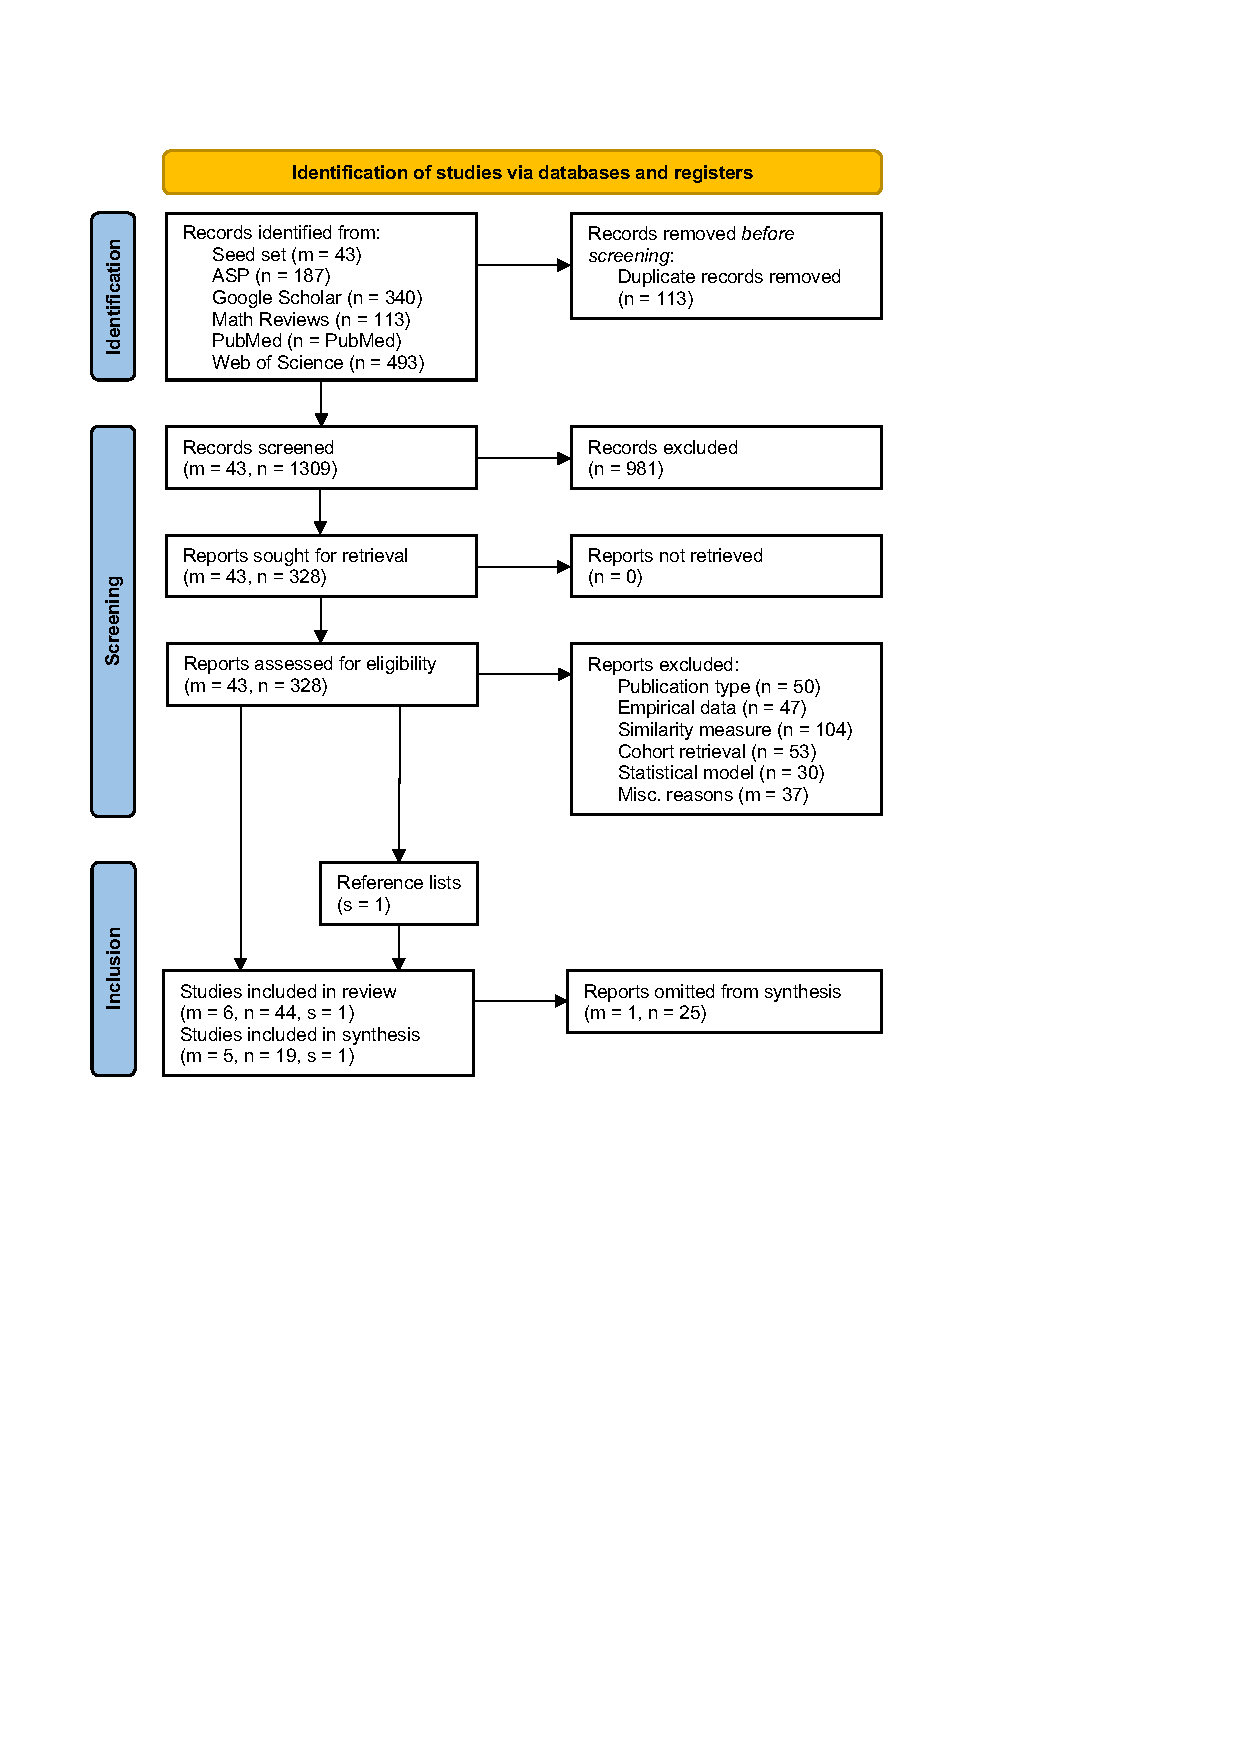
\includegraphics[width=0.8\linewidth]{Fig1} 

}

\caption{PRISMA-S flow chart. Lowercase letters refer to items obtained from the seed set (m), the structured search (n), and citation/reference tracking (s). Within the structured search results, summands correspond to original and update.}\label{fig:prisma}
\end{figure}

From the first search results, there were 60 disagreements over
inclusion versus exclusion. Inter-rater reliability was low, at 82\%
relative to a 72\% probability of random agreement. Only one author was
available to review full texts from the update search.

We then reviewed 43 studies comprising a seed set that inspired this
review. After removing duplicates and screening for eligibility, we were
left with 6 additional studies (Park, Kim, and Chun 2006; Lowsky et al.
2013; Lee, Maslove, and Dubin 2015; Ng et al. 2015; Lee 2017; N. Wang et
al. 2019), 1 of which was excluded from the synthesis for using NN
prediction. Reference tracking from the 43 + 360 = 403 studies assessed
for eligibility led us to identify 1 additional study that met our
criteria (Kasabov and Hu 2010). This left us with 21 + 1 + 5 = 27
studies included in the review and synthesis.

\hypertarget{bibliographic-and-methodological-properties}{%
\subsection{Bibliographic and methodological
properties}\label{bibliographic-and-methodological-properties}}

The 27 included studies were analyzed based on several characteristics,
and we report and describe some observations here (Table
\ref{tab:synthesis}). The studies were published in a variety of
journals, with some of greater frequency, though no single journal
published more than 3. The journal \emph{Evolving Systems} published 2
of the included studies, \emph{Artificial Intelligence in Medicine}
published 3, \emph{Hindawi - Journal of Healthcare Engineering}
published 3, \emph{Evolving Systems} published 2, and \emph{PLOS One}
published 2.

Another interesting pattern lay in the years of publication (Figure
\ref{fig:year}). While these studies trace back to the late 1990s, they
have become more common, which suggests that this is an active, though
not rapidly expanding, approach. We note that CBR in health and medicine
originated as early as 1990, and localized modeling emerged soon after
CBR had established itself; the idea has been ``in the air'' for as long
as CBR has been in use.

\small

\begin{longtable}[]{@{}
  >{\raggedright\arraybackslash}p{(\columnwidth - 12\tabcolsep) * \real{0.1148}}
  >{\raggedright\arraybackslash}p{(\columnwidth - 12\tabcolsep) * \real{0.1585}}
  >{\raggedright\arraybackslash}p{(\columnwidth - 12\tabcolsep) * \real{0.1202}}
  >{\raggedright\arraybackslash}p{(\columnwidth - 12\tabcolsep) * \real{0.1967}}
  >{\raggedright\arraybackslash}p{(\columnwidth - 12\tabcolsep) * \real{0.1530}}
  >{\raggedleft\arraybackslash}p{(\columnwidth - 12\tabcolsep) * \real{0.1038}}
  >{\raggedleft\arraybackslash}p{(\columnwidth - 12\tabcolsep) * \real{0.1530}}@{}}
\caption{\label{tab:synthesis}Studies included in the method synthesis,
arranged by the earliest the study is known to have been
public.}\tabularnewline
\toprule\noalign{}
\begin{minipage}[b]{\linewidth}\raggedright
Citation
\end{minipage} & \begin{minipage}[b]{\linewidth}\raggedright
Task
\end{minipage} & \begin{minipage}[b]{\linewidth}\raggedright
Aim
\end{minipage} & \begin{minipage}[b]{\linewidth}\raggedright
Source
\end{minipage} & \begin{minipage}[b]{\linewidth}\raggedright
Type
\end{minipage} & \begin{minipage}[b]{\linewidth}\raggedleft
Cases
\end{minipage} & \begin{minipage}[b]{\linewidth}\raggedleft
Features
\end{minipage} \\
\midrule\noalign{}
\endfirsthead
\toprule\noalign{}
\begin{minipage}[b]{\linewidth}\raggedright
Citation
\end{minipage} & \begin{minipage}[b]{\linewidth}\raggedright
Task
\end{minipage} & \begin{minipage}[b]{\linewidth}\raggedright
Aim
\end{minipage} & \begin{minipage}[b]{\linewidth}\raggedright
Source
\end{minipage} & \begin{minipage}[b]{\linewidth}\raggedright
Type
\end{minipage} & \begin{minipage}[b]{\linewidth}\raggedleft
Cases
\end{minipage} & \begin{minipage}[b]{\linewidth}\raggedleft
Features
\end{minipage} \\
\midrule\noalign{}
\endhead
\bottomrule\noalign{}
\endlastfoot
Yearwood and Wilkinson (1997) & Prediction\hspace{6em} &
Practice\hspace{6em} & Clinical\hspace{6em} &
Cross-sectional\hspace{6em} & 1,355 & 9 \\
Mariuzzi et al. (1997) & Prognosis\hspace{6em} & Knowledge\hspace{6em} &
Clinical\hspace{6em} & Longitudinal\hspace{6em} & 113 & 4 \\
Wyns et al. (2004) & Prediction\hspace{6em} & Practice\hspace{6em} &
Laboratory\hspace{6em} & Cross-sectional\hspace{6em} & 160 & 14 \\
Park, Kim, and Chun (2006) & Diagnosis\hspace{6em} &
Practice\hspace{6em} & Clinical, Imaging\hspace{6em} &
Cross-sectional\hspace{6em} & 366; 270; 560; 760 & 35; 14; 31; 8 \\
Song and Kasabov (2006) & Prediction\hspace{6em} & Practice\hspace{6em}
& Clinical\hspace{6em} & Cross-sectional\hspace{6em} & 1,000; 447 & 6;
6 \\
Elter, Schulz-Wendtland, and Wittenberg (2007) & Prediction\hspace{6em}
& Practice\hspace{6em} & Clinical\hspace{6em} &
Cross-sectional\hspace{6em} & 2,620 & 6 \\
Xu et al. (2008) & Prediction\hspace{6em} & Practice\hspace{6em} &
Clinical\hspace{6em} & Cross-sectional\hspace{6em} & 67 & 14 \\
López et al. (2011) & Diagnosis\hspace{6em} & Knowledge\hspace{6em} &
Clinical\hspace{6em} & Cross-sectional\hspace{6em} & 871 & 4 \\
Kasabov and Hu (2010) & Diagnosis\hspace{6em} & Knowledge\hspace{6em} &
Clinical\hspace{6em} & Cross-sectional\hspace{6em} & 62 & 2,000 \\
Verma et al. (2015) & Decision Support\hspace{6em} &
Practice\hspace{6em} & Clinical\hspace{6em} &
Cross-sectional\hspace{6em} & 74 & 93 \\
Liang, Hu, and Kasabov (2015) & Prediction\hspace{6em} &
Practice\hspace{6em} & Clinical\hspace{6em} &
Cross-sectional\hspace{6em} & 62; 72; 77; 181 & 2,000; 7,129; 7,129;
12,533 \\
Lowsky et al. (2013) & Prediction\hspace{6em} & Practice\hspace{6em} &
Clinical, Laboratory\hspace{6em} & Longitudinal\hspace{6em} & 13,525 &
13 \\
Campillo-Gimenez et al. (2013) & Decision Support\hspace{6em} &
Practice\hspace{6em} & Patient-reported\hspace{6em} &
Cross-sectional\hspace{6em} & 1,647 & 18 \\
Nicolas et al. (2014) & Diagnosis\hspace{6em} & Knowledge\hspace{6em} &
Clinical\hspace{6em} & Cross-sectional\hspace{6em} & 150 & 83 \\
Ng et al. (2015) & Clustering\hspace{6em} & Practice\hspace{6em} &
Clinical, Laboratory\hspace{6em} & Longitudinal\hspace{6em} & 7,519 &
130 \\
Lee, Maslove, and Dubin (2015) & Prediction\hspace{6em} &
Knowledge\hspace{6em} & Clinical, Laboratory\hspace{6em} &
Cross-sectional\hspace{6em} & 17,152 & 75 \\
Vilhena et al. (2016) & Diagnosis\hspace{6em} & Knowledge\hspace{6em} &
Clinical\hspace{6em} & Cross-sectional\hspace{6em} & 1,046 & 8 \\
Lee (2017) & Prediction\hspace{6em} & Practice\hspace{6em} & Clinical,
Laboratory\hspace{6em} & Cross-sectional\hspace{6em} & 17,152 & 75 \\
Zhang et al. (2018) & Diagnosis\hspace{6em} & Knowledge\hspace{6em} &
Imaging\hspace{6em} & Cross-sectional\hspace{6em} & 810; 302 & 8 \\
Malykh and Rudetskiy (2018) & Decision Support\hspace{6em} &
Practice\hspace{6em} & Clinical\hspace{6em} &
Cross-sectional\hspace{6em} & 638 & 49,728 \\
Ma et al. (2020) & Prediction\hspace{6em} & Practice\hspace{6em} &
Clinical\hspace{6em} & Cross-sectional\hspace{6em} & 4,000 & 22 \\
N. Wang et al. (2019) & Diagnosis\hspace{6em} & Practice\hspace{6em} &
Clinical, Laboratory\hspace{6em} & Cross-sectional\hspace{6em} & 16,490
& 106 \\
Y. Wang et al. (2020) & Decision Support\hspace{6em} &
Practice\hspace{6em} & Clinical\hspace{6em} &
Cross-sectional\hspace{6em} & 8 & 5 \\
Tang et al. (2021); Ng et al. (2021) & Decision Support\hspace{6em} &
Practice\hspace{6em} & Clinical\hspace{6em} & Longitudinal\hspace{6em} &
245,825 & 1,466,474 \\
Liu et al. (2022) & Prediction\hspace{6em} & Practice\hspace{6em} &
Clinical, Laboratory\hspace{6em} & Cross-sectional\hspace{6em} & 76,597
& 1,892 \\
Doborjeh et al. (2022) & Prediction\hspace{6em} & Practice\hspace{6em} &
Clinical, Environmental\hspace{6em} & Longitudinal\hspace{6em} & 804 &
46 \\
\end{longtable}

\normalsize

\begin{figure}

{\centering 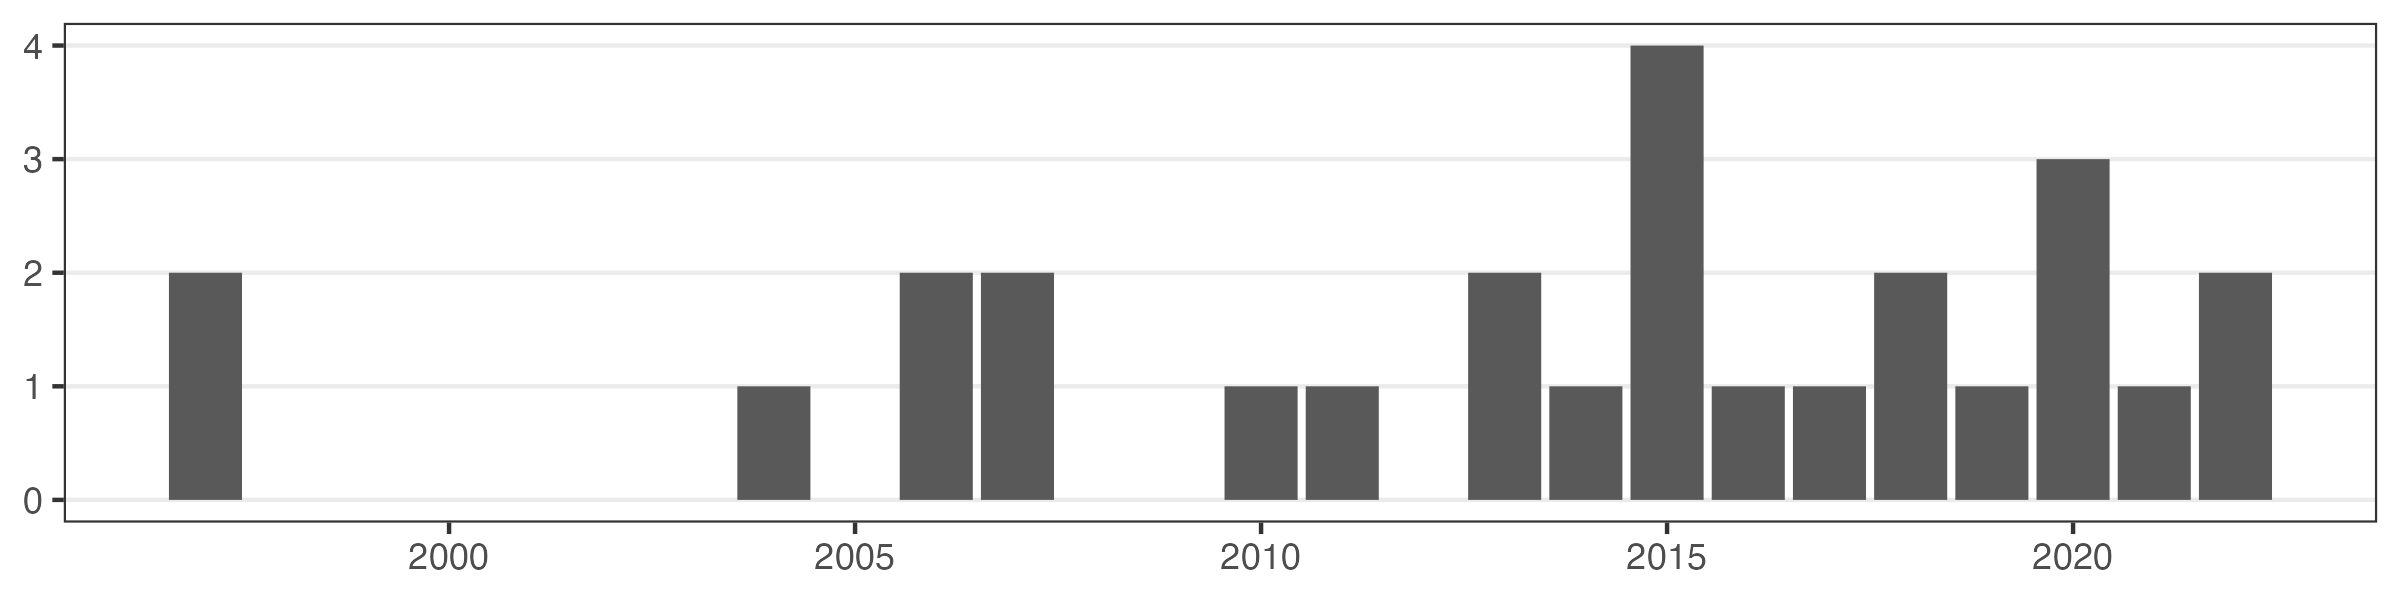
\includegraphics[width=1\linewidth]{Fig2} 

}

\caption{Number of publications in our sample each year.}\label{fig:year}
\end{figure}

Another dominant characteristic of included studies is their broader
remit. We categorized studies as ``knowledge'' or ``practice'' based on
whether their aim was to produce generalizable knowledge or to improve
practice. We classified 8 of the studies as ``knowledge'', making the
majority of studies from a ``practice'' standpoint. These studies aimed
to provide tools for use in clinic or to improve outcomes.

Lastly, we observed a commonality among 6 of the included studies in
having evaluated methods using leave-one-out cross-validation (LOOCV).
The purpose of this measure is to estimate the overall performance of
certain factors when used to make predictions, particularly utilized on
smaller data sets, where models benefit greatly from larger training
sets and additional model fitting is less costly.

In addition to the aim of its analysis, we coded several aspects of the
design of each study, including the source and type of data and the
clinical task the model performed (Table \ref{tab:synthesis}), as well
as the specific methodology and terminology adopted (Table
\ref{tab:composite}). In the following subsections, we take a closer
look at these design elements and their reported justifications and
limitations.

\hypertarget{application-domains}{%
\subsection{Application domains}\label{application-domains}}

While all included studies were reported in scientific and medical
journals, the vast majority were oriented toward clinical practice
rather than medical research. For example, a 2006 study specifically
evaluated the usefulness of CBR-based explanations for the purpose of
decision support (Doyle, Cunningham, and Walsh 2006). This study was
part of a much larger literature on CBR systems and was included here
despite relying on NN prediction because it used an unconventional
voting scheme to generate recommendations. A more recent study took
essentially the same focus with respect to a proposed clinical risk
prediction model, which amounted to CBR with a novel weighting scheme on
predictors informed by expert consensus (Fang et al. 2021). In both
cases a prototype implementation was deployed in an experimental setting
for evaluation.

The most common clinical motivations were individualized detection or
diagnosis, prognosis or outcome prediction, and treatment or care
recommendation. The plurality focused on prognosis or outcome
prediction, often using time-to-event analysis: Mariuzzi et al. (1997)
used CBR to predict survival time from several geometric properties of
breast tumors. Lowsky et al. (2013) used CBR with non-parametric
survival models on registry data to predict patient--graft survival
times following kidney transplantation. Lee, Maslove, and Dubin (2015)
and Lee (2017) used localized logistic regression and random forest
modeling to predict 30-day mortality following discharge for ICU
patients. Vilhena et al. (2016) developed a CBR cycle around a
clustering-informed similarity matching procedure and an artificial
neural network--based classifier to identify thrombophilia patients at
high risk of thrombotic episodes. Ma et al. (2020) took a similarity
cohort--based approach to predicting length of stay for ICU patients.
Doborjeh et al. (2022) localized spiking neural networks in order to
assess stroke risk from up to 7-day time series of clinical and
environmental factors. Liu et al. (2022) incorporated global-to-local
transfer learning into localized models of acute kidney injury risk in
hospitalized patients. Also of note, from a public health perspective,
Xu et al. (2008) used CBR to predict rehabilitation time as well as
disability risk for unemployed workers experiencing chronic pain.

Toward detection and diagnosis, Wyns et al. (2004) proposed a hybrid
neural net--CBR system to distinguish (with confidence bounds) arthritic
versus control patients, based on several histological features. Nicolas
et al. (2014) used collaborative multilabel CBR to subtype melanoma
patients based on confocal and dermoscopy images. N. Wang et al. (2019)
used localized models built from a multi-type additive similarity
measure to distinguish type 2 diabetic versus control populations. Along
the way, Song and Kasabov (2006), Kasabov and Hu (2010), and Verma et
al. (2015) took an iterative model-building approach to several tasks:
predicting glomerular filtration rate, a key indicator of renal
function, from demographic and physiological variables; identifying
patients with colon cancer using a large number of gene expression
measurements; and identifying patients with type 2 diabetes based on
demographic, physiological, and genetic variables.

While several studies emphasized the potential or actual value to
decision-making of their methods and tools, only one incorporated
treatment decisions into their approach: By taking ``decision points''
as their units of analysis, Tang et al. (2021) and Ng et al. (2021)
built not classifiers or predictors but comparative effectiveness models
into a localized framework, providing for the first time in our sample
explicitly prescriptive rather than descriptive clinical decision
support.

A partial exception to this focus was a 2014 study that also reported a
decision support tool, in this case for early diagnosis of melanoma from
clinical data and dermoscopy images (Nicolas et al. 2014). While the
stated objectives were analogous, specific emphasis was placed on the
acquisition of new knowledge through the development of the tool,
including the systematic generation of new data and creation of a
clinical ontology. This study was included for its use of a
collaborative classifier that drew from multiple modeling approaches. In
keeping with this focus of the included literature, the stated
objectives of the proposed methods were more often (or additionally) to
predict outcomes or to recommend interventions than only to diagnose
disease.

The mosaic plot in Figure \ref{fig:properties} summarizes the relation
between data source, clinical task, and aim.

\begin{figure}

{\centering 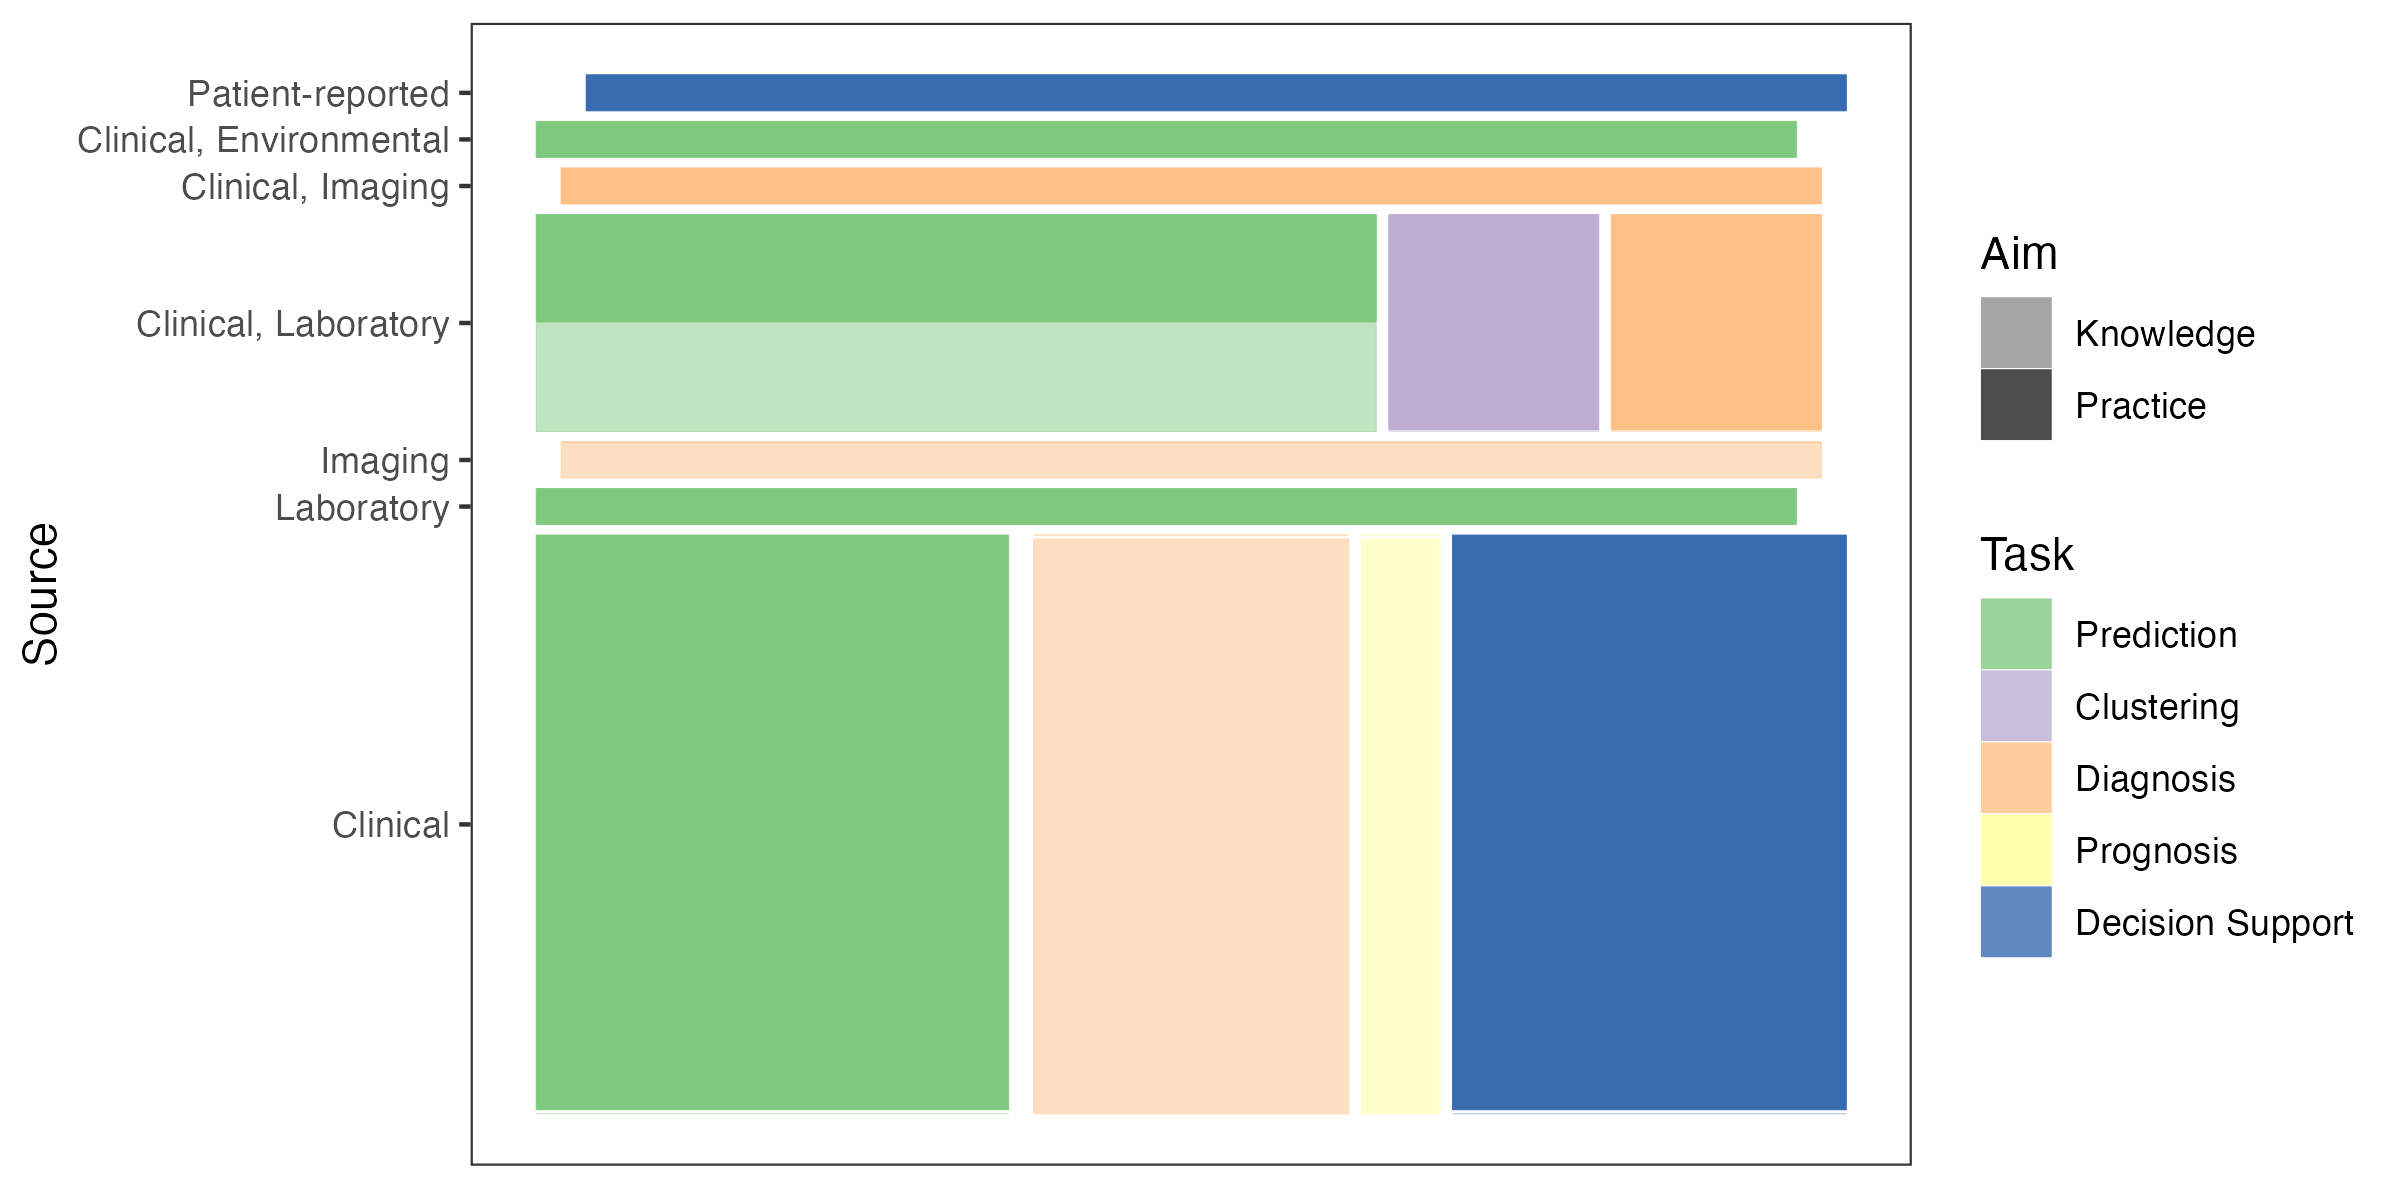
\includegraphics[width=1\linewidth]{Fig3} 

}

\caption{Share of studies characterized by several design elements: data source (row), clinical task (fill), and remit (opacity).}\label{fig:properties}
\end{figure}

\hypertarget{rationales}{%
\subsection{Rationales}\label{rationales}}

The included studies hypothesized, asserted, or assumed several benefits
of localized modeling specific to clinical and medical settings and
advantages over other modeling approaches. The most common was that the
restriction to similar or relevant past cases would improve predictive
performance for the index case (Mariuzzi et al. 1997; Liang, Hu, and
Kasabov 2015; Ng et al. 2015; Lee 2017). In particular, Lee, Maslove,
and Dubin (2015) hypothesized and confirmed that the value of each past
case would be positively related to its similarity to the index case, an
assumption built in to the weighting schemes of other approaches. Lowsky
et al. (2013) made a different case, that the fewer parametric
assumptions and complications of a CBR-style model would allow for
greater accuracy. Additionally, several investigators asserted that the
use of localized cohorts befit the clinical focus on the individual
patient rather than the population, without reference to performance
(Song and Kasabov 2006; Xu et al. 2008).

In an interesting contrast, Tang et al. (2021) and Ng et al. (2021)
argued that their localized approach using the larger and more
heterogeneous populations covered by EHR-derived data could better
capture the messy and diverse lessons of everyday practice, as a
counterpart to guidelines based on randomized controlled trials. Their
emphasis on the enabling role of EHRs to power methods well-suited to
large, structured data repositories was shared by several others
(Campillo-Gimenez et al. 2013; Nicolas et al. 2014; Verma et al. 2015;
Lee 2017). Verma et al. (2015) and Zhang et al. (2018) additionally
pointed out that localized models are adaptable to noise in the data,
variation in patterns of missingness, and (harkening to the last step of
the R4 cycle) addition of new cases with known outcomes to the corpus.
These properties, they said, tend to be more difficult for
whole-population models to handle.

The other frequent advantage attributed to localized modeling was
interpretability. Elter, Schulz-Wendtland, and Wittenberg (2007) and
Nicolas et al. (2014) emphasized the value of the detailed past cases,
available to the user, on which predictions are based. This
``self-explanation capability'' made outputs more intelligible to
physicians in the CDS setting. Ng et al. (2015) additionally pointed out
that localized GLMs yield localized effect estimates, which may help
investigators identify individually relevant risk factors. Liu et al.
(2022) took this idea further, systematically comparing regression
coefficients for specific risk factors across dozens of diagnostic
subpopulations. Doborjeh et al. (2022) used localized time series models
to identify environmental changes associated with increased stroke risk.

The remaining coded rationales were for augmentations or hybridizations
of then-conventional CBR, most of which defended the use of other tools
to improve performance via cohort selection (Campillo-Gimenez et al.
2013; Nicolas et al. 2014; Vilhena et al. 2016) or to make models and
outputs more interpretable (López et al. 2011; N. Wang et al. 2019).
Liang, Hu, and Kasabov (2015) argued for simultaneous optimization of
cohort and feature selection with model parameterization; their TWNFI
approach combines localization with regularization.

\hypertarget{challenges}{%
\subsection{Challenges}\label{challenges}}

CBR can be understood as the opposite side of a trade-off with
rule-based reasoning between model size and model complexity: Doyle,
Cunningham, and Walsh (2006) describe their approach as
``knowledge-light'', in that ``the cases do not contain explicit
explanation structures; instead, explanation is achieved by comparison
of the query case with retrieved cases''. This means that the greatest
performance and efficiency challenges in CBR have to do with the
retrieval and revision phases in the R4 cycle. Several studies addressed
these challenges: Park, Kim, and Chun (2006), while excluded from the
synthesis, were the earliest to propose that cohorts be bounded by a
similarity threshold rather than by the number of cases, which improved
performance in their experiments. Campillo-Gimenez et al. (2013)
leveraged predictor weights obtained from logistic regression to inform
the similarity calculation used in retrieval. Lowsky et al. (2013) used
non-parametric models to reduce the computational burden of revision
(prediction). Ma et al. (2020) proposed to improve efficiency along the
entire R4 cycle, but in particular by only executing task-dependent
steps in real time (``just-in-time learning'', JITL), and Ng et al.
(2021) and Tang et al. (2021) partitioned multiple phases in the R4
cycle into offline and online components, only the latter of which would
be performed in real time as new data are received. Liu et al. (2022)
used transfer learning from globally-fitted models to improve the
efficiency of localized models.

Other studies addressed limitations of available tools. López et al.
(2011) implemented a comprehensive CBR tool in response to the lack of
general-purpose software, to enable coupling with other tools as well as
to expedite development, experimentation, and uptake. Several other
teams also set out to develop more generalizable and data-agnostic
clinical support tools (Elter, Schulz-Wendtland, and Wittenberg 2007;
Liang, Hu, and Kasabov 2015; Ng et al. 2015; Zhang et al. 2018).
However, more informatical and legal challenges to implementation,
including interoperability of systems and data and regulations
concerning security and privacy, were rarely addressed. We discuss this
further in Section \ref{feasibility}.

Figure \ref{fig:methods} compares the rates at which several
methodological elements are invoked in the sample.

\hypertarget{evaluations}{%
\subsection{Evaluations}\label{evaluations}}

Most included studies quantitatively compared the predictive performance
of their proposed method(s) to one or more comparators. What we took to
be the signature results are collated in Table \ref{tab:performance} in
the Appendix. Note that we exercised some judgment in classifying
methods as proposals and comparators, as in some cases all methods were
original but only some showcased main ideas. It would be impractical to
meta-analyze these numbers due to the great variety of settings,
problems, data types, techniques, and choices involved.

We do observe one clear pattern: All of the proposed methods that most
evidently outperformed their comparators---Kohonen + CBR (Wyns et al.
2004), TWNFI Kasabov and Hu (2010), gravitational search algorithms
(GSA) (Liang, Hu, and Kasabov 2015), CBR + rules (+ DML) (Nicolas et al.
2014), Gaussian process regression (Zhang et al. 2018), JITL-ELM (Ma et
al. 2020)---are hybrids of localized modeling (in some cases CBR) with
other techniques, often DML. Though Campillo-Gimenez et al. (2013) and
Ng et al. (2015) report non-superior performance by such hybrids, the
pattern suggests the importance of the similarity measure to the
retrieval step. Meanwhile, when proposed approaches targeted cohort
demarcation or choice of predictive model---statistical CBR (Park, Kim,
and Chun 2006); individualized logistic regression, decision tree, and
random forest (Lee, Maslove, and Dubin 2015; Lee 2017)---they did not
consistently outperform comparators.

\hypertarget{identified-needs}{%
\subsection{Identified needs}\label{identified-needs}}

The study authors focused their recommendations and their own plans for
future work mostly on technical improvements and evaluations (Mariuzzi
et al. 1997; Yearwood and Wilkinson 1997). Urged improvements included
full or partial automation of predictor selection (Mariuzzi et al. 1997;
Yearwood and Wilkinson 1997), similarity learning (Mariuzzi et al. 1997;
N. Wang et al. 2019), and parameter optimization (Song and Kasabov 2006;
Lee 2017); extensions to new data structures (López et al. 2011), data
types (Liang, Hu, and Kasabov 2015; Verma et al. 2015; Malykh and
Rudetskiy 2018), and reasoning systems (Nicolas et al. 2014); and the
use of more advanced model components to improve accuracy or efficiency
(Lowsky et al. 2013; Lee, Maslove, and Dubin 2015; Liang, Hu, and
Kasabov 2015; Zhang et al. 2018). Authors also urged validations and
independent evaluations using larger or more comprehensive data sets
(Elter, Schulz-Wendtland, and Wittenberg 2007; Xu et al. 2008; Verma et
al. 2015; Ng et al. 2015), using data aggregated from multiple health
systems (Lee, Maslove, and Dubin 2015; Lee 2017; Tang et al. 2021; Ng et
al. 2021), and in other care settings or disease contexts (Song and
Kasabov 2006; Zhang et al. 2018; Tang et al. 2021; Ng et al. 2021).

Less common were calls to strengthen the connection between the methods
and the users. Some authors urged the incorporation of (human-derived)
domain knowledge into the data or models (Yearwood and Wilkinson 1997;
N. Wang et al. 2019). Others suggested new uses of their modeling
approaches: to measure feature importance (Wyns et al. 2004), to make
models more expressive (Lee, Maslove, and Dubin 2015), and to combine
information obtained both from global and from localized models (Ng et
al. 2015). Most of this incremental work was indeed carried out in later
investigations in our sample. That said, we did not find reports of
successful implementations of these tools in clinical practice. (Several
excluded studies did showcase uses of CBR in practice.)

\hypertarget{discussion}{%
\section{Discussion}\label{discussion}}

After commenting briefly on our review process, we draw several
observations from our encoding of the included studies. We first focus
on their methodological choices and innovations, then on their
conventions and language. We spend most of the section discussing the
differences and commonalities of the techniques used, toward a general
method that encompasses most or all cases. We then suggest some avenues
for future studies and conclude with our key takeaways.

\hypertarget{process}{%
\subsection{Process}\label{process}}

The low inter-rater reliability was due, in parts, to different
interpretations of some eligibility criteria by the authors,
inconsistent terminology across the sample, and incomplete reporting of
resources and methods in the sample. Regarding interpretation of
criteria, some wording of the criteria was adjusted following
discussions between the reviewing authors during full-text review to
better specify an agreed-upon meaning. We will discuss the different
domains, terminologies, and reporting issues of the sample in the
remainder of this section.

\hypertarget{study-designs}{%
\subsection{Study designs}\label{study-designs}}

Consistent with their orientation, almost all included studies were
conducted using clinical data, only occasionally together with
patient-reported (2), laboratory (3), image (1), and environmental (1)
data. We suggest three reasons for this: First, this literature traces
back to the 1990s, before -omic data could be generated cost-effectively
at scale. Second, CBR in particular has a strong tradition in clinical
decision support, where the focus of our sample remains throughout the
review period. Third, because most -omic data are highly
homogeneous---all measurements are made along or can be transformed to a
common scale, e.g.~greyscale pixellations for X-ray images and
transcripts per million for RNA-seq data---more deeply theoretical
analysis techniques have been developed and come into wide use. While
variations on correlation-based approaches like EHR-based phenome-wide
association studies and similarity-based methods like CBR itself have
been developed, more mechanistic and probabilistic tools have not become
a domain standard.

Because we excluded studies that used conventional NN prediction, many
included studies reported new approaches to adaptation subsequent to
retrieval. Very few proposed novel similarity measures, possibly because
larger studies tended to be reported in separate articles detailing
experiments with specific components of the process. However, this also
suggests that few experimental studies have focused on the unified
development of new retrieval and adaptation strategies. We also note
that the majority of studies evaluated and compared methods using
leave-one-out cross-validation (LOOCV). This is an appropriate technique
when available data are scarce, and indeed most data sets used by
included studies numbered in the hundreds of cases or fewer. This likely
follows from the older age of many included studies and from their
consistent primary focus on clinical data, which is more costly to
collect and comes with more restrictions on its use.

\hypertarget{coherence}{%
\subsection{Coherence}\label{coherence}}

The motivational and methodological unity of these studies does not
reflect a unified research program. Besides the lack of any primary
journal of record, we observed collaborations only among the authors of
smaller contiguous programs, including applications of the TWNFI
methodology (Song and Kasabov 2006; Verma et al. 2015), individualized
mortality prediction for ICU patients (Lee, Maslove, and Dubin 2015; Lee
2017) and the use of more explanatory models to prioritize predictors or
treatments for chronic disease (Ng et al. 2015; Tang et al. 2021; Ng et
al. 2021).

These programs used varying terminology for common concepts, and no
common term is in use for what we here refer to as localized modeling;
authors described their approaches as ``targeted prognosis'' (Mariuzzi
et al. 1997), ``transductive inference'' (Song and Kasabov 2006),
``personalized decision support'' (Lee, Maslove, and Dubin 2015),
``personalized (predictive) models'' (Liang, Hu, and Kasabov 2015, in
contrast to ``local models''; Ng et al. 2015; N. Wang et al. 2019; Ma et
al. 2020; Liu et al. 2022; Doborjeh et al. 2022), and ``precision
cohort'' analysis (N. Wang et al. 2019; Tang et al. 2021; Ng et al.
2021). We find uses of ``targeted'', ``personalized'', and ``precision''
generic and imprecise, while transductive inference is an established
term for a broader set of methods in ML. Because \emph{local} naturally
contrasts with \emph{global}, we propose ``localized models'' as a
suitable term for this counterpart to globally-fitted models.\footnote{We
  note, in response to one reviewer's comment, that for many if not most
  models used in ML, excepting GLMs, a predictor may play a different
  and more or less important role for some cases than others, as
  quantified by importance measures or model-agnostic explanations
  (Biecek and Burzykowski 2021; Molnar 2023). In this way, such models
  can also be viewed as ``localized''. We recognize that the use of
  global and local explanations is standard. As another reviewer pointed
  out, the terminology of local and global is also used in the unrelated
  context of federated ML to distinguish models trained using data
  stored in a single storage device (local) from their aggregations
  (global) (Moshawrab et al. 2023; Brauneck et al. 2023). The prospects
  for federated architecture to more effectively implement similarity
  cohort--based models are intriguing, and would require some
  reconciliation of terms. At present, we feel that these methods are
  sufficiently disjoint to avoid confusion in practice, but we suggest
  the more specific term ``similarity cohort--based models'' when the
  term ``local'' is overloaded.}

\hypertarget{synthesis-1}{%
\subsection{Synthesis}\label{synthesis-1}}

The 27 studies included in our synthesis used composite techniques that
we organized into two major types. One type, \emph{similarity learning},
was used in 8 studies that tie in to the much larger literature on DML
(Yang 2006). The other, \emph{cohort thresholding}, focused on choosing
or optimizing the manner in which cohorts were demarcated using the
similarity measure.

\hypertarget{similarity-learning-and-threshold-optimization}{%
\subsubsection{Similarity learning and threshold
optimization}\label{similarity-learning-and-threshold-optimization}}

The similarity learning approaches took a variety of forms. These
techniques are designed to detect structure in data, especially
associations between predictors and responses, and to use this structure
to inform the definition of a patient similarity measure. Eight studies
used response values in training data sets to supervise similarity
learning while two used unsupervised learning (Table
\ref{tab:composite}). Based on the key properties of DML algorithms
identified by Bellet, Habrard, and Sebban (2014), most learned measures
were non-linear while some were locally learned, and some were optimized
globally while others locally. Not all qualified as DML, since the
resulting measures would not necessarily satisfy the triangle
inequality. Each used its similarity measure to retrieve training cases
relevant to each testing case. Once retrieved, most took a standard NN
approach to generating predictions; two exceptions (Vilhena et al. 2016;
Tang et al. 2021) fit predictive models to the retrieved cohorts.

Several studies used unsupervised similarity learning, for example the
Mahalanobis distance (Lowsky et al. 2013) and the Kolmogorov
entropy-based distance (Elter, Schulz-Wendtland, and Wittenberg 2007).
In particular, Yearwood and Wilkinson (1997) defined similarity as a
weighted sum of differences in predictor values and used linear
regression to optimize the weights for the predictive accuracy of the
cohort they retrieve. Others used supervised learning: Song and Kasabov
(2006) proposed an iterative algorithm to optimize a set of fuzzy
inference rules used to retrieve relevant cases and generate a
prediction, using back-propagation on the rules' parameters. Their
method was used in several later studies returned by our search, which
are not discussed here because they did not originate the technique.
Nicolas et al. (2014) explicitly appeal to a supervised distance metric
learning (DML) technique (Xing et al. 2002) to obtain a similarity
measure on their set of dermoscopy and confocal images that most
effectively separates malignant from benign melanoma tumors. We will
discuss the remaining uses of supervised similarity learning shortly.

Distinct from but related to similarity learning was supervised cohort
construction. This was an adaptive step taken by Park, Kim, and Chun
(2006) to optimize the predictive performance of models fitted to
cohorts retrieved using a fixed similarity rather than count threshold,
a counterpart to conventional CBR they called ``statistical
CBR''.\footnote{Drawing from Goyal, Lifshits, and Schütze (2008), we
  suggest the term ``combinatorial CBR'' for the then-conventional
  approach using similarity cohorts of fixed cardinality.} The step used
a heuristic procedure to locate a similarity threshold that (locally)
maximizes predictive accuracy on the training set. This is analogous to
optimizing the neighborhood size parameter in NN predictive modeling, so
we will not discuss it further except to mention that the authors found
statistical CBR to outperform conventional CBR on several data sets.
Campillo-Gimenez et al. (2013) combined these learning techniques: They
used logistic regression on the training set to obtain weights for the
predictors (by predicting the binary outcome of kidney transplant
waitlist registration) and for the cases (by predicting agreement of
outcome between an index case and other training cases), and they used
exhaustion to optimize the size of the retrieved cohort for the accuracy
of the NN model using the previously optimized weights.

As noted above, these instances of similarity learning fit into a much
larger literature on DML, which has seen widespread use in health
informatics and modeling. That these studies satisfied our review
criteria is due to the novelty of the techniques at the time of
publication and the detailed attention paid to their techniques by the
authors. It also reflects a limitation of our study and of the
literature we set out to retrieve: We are aware of no standard terms in
use to identify the family of techniques that fit statistical models to
similarity-based cohorts. The retrieved studies whose use of such
techniques alone satisfied our criteria variably termed them
individualized, personalized, local, and patient-specific models, among
other terms (Table \ref{tab:composite}). We prefer the term localized
models, which is both sensitive and specific to uses of a similarity or
distance measure to retrieve a cohort to which a model is fit: It
includes some properly included techniques we did not have in mind
(Vilhena et al. 2016) yet excludes other techniques commonly referred to
as individualized, personalized, or precision.

\hypertarget{localized-models}{%
\subsubsection{Localized models}\label{localized-models}}

In addition to Lowsky et al. (2013), Liang, Hu, and Kasabov (2015), Ng
et al. (2015), Lee (2017), Vilhena et al. (2016), Tang et al. (2021),
and Ng et al. (2021), seven other studies employed localized models:
Mariuzzi et al. (1997), Lee, Maslove, and Dubin (2015), Verma et al.
(2015), N. Wang et al. (2019), Ma et al. (2020), Liu et al. (2022), and
Doborjeh et al. (2022). In most cases these models were purely
predictive in application; of the exceptions, Mariuzzi et al. (1997)
produced purely descriptive models of survival outcomes, which were
evaluated for their precision rather than their accuracy, while Ng et
al. (2015) used generalized regression models descriptively as well as
predictively, as did Tang et al. (2021), Ng et al. (2021), and Liu et
al. (2022) later. The most common approach to cohort selection was to
optimize a size threshold via manual exploration (Mariuzzi et al. 1997;
Lee, Maslove, and Dubin 2015; Ng et al. 2015; Lee 2017; N. Wang et al.
2019; Vilhena et al. 2016) or via cross-validation (Lowsky et al. 2013;
Verma et al. 2015). Further in the former direction, one study (Ma et
al. 2020) set a fixed cohort size while two (Liang, Hu, and Kasabov
2015; Tang et al. 2021; Ng et al. 2021) devised more sophisticated
algorithms to balance multiple desiderata including predictive accuracy.

Several themes emerged from this sample. Foremost was the optimization
of retrieved cohort sizes for some measure of model performance. Despite
the early recommendation by Park, Kim, and Chun (2006) to threshold
cohorts by similarity rather than by cardinality, only the one
previously published study (Mariuzzi et al. 1997) and the most recent
study (Tang et al. 2021; Ng et al. 2021) in this corpus took this
approach, though Liu et al. (2022) took a third option by retrieving
fixed proportions of training data. Viewed as a hyperparameter of the
individualized modeling approach, cohort size can be treated in the same
way as neighborhood size in NN prediction (viewed here as a special case
of localized modeling wherein the model is a simple summary statistic),
so we will not discuss it further.

An alternative approach was to optimize multiple hyperparameters
together: Kasabov and Hu (2010) proposed an iterative algorithm to
settle on an optimal number and set of predictors as well as number of
training cases (comprising the retrieved cohort) that was later used by
Liang, Hu, and Kasabov (2015). More recently, Tang et al. (2021) and Ng
et al. (2021) proposed a three-step process for cohort selection that
filtered by exact match for one subset of predictors, used
domain-informed similarity measures to rank these, and optimized the
similarity threshold for a trade-off between cohort size and a measure
of bias called cohort balance. Notably, though their similarity measure
was supervised, this optimization process was not.

With the exception of the descriptive survival models of Mariuzzi et al.
(1997), only one thread in this corpus concerned itself with the
interpretability of localized models: Ng et al. (2015) fit logistic
regression models to similarity-based cohorts and examined not only
their predictive performance but the localized sets of largest and most
detectable predictors, termed risk profiles, and how they differed
across the testing population. This approach informed their later use of
localized comparative effectiveness--style models to recommend courses
of treatment at decision points during a monitored patent's stay (Tang
et al. 2021; Ng et al. 2021), and it was later used by Liu et al. (2022)
to show a dependency of predictor importance on the patient disease
subgroup. These studies suggest much wider potential for localized
real-world evidence generation, which has long been promoted as a
promise of advances in clinical and health informatics (Longhurst,
Harrington, and Shah 2014).

\hypertarget{a-general-framework}{%
\subsubsection{A general framework}\label{a-general-framework}}

This relatively small sample exhibited a wide range of approaches, both
technically and conceptually. Discussion of the technical diversity of
these approaches has been summarized above and published in greater
detail in previous reviews (Choudhury and Begum 2016; Sharafoddini,
Dubin, and Lee 2017; Parimbelli et al. 2018), and we focus here on the
conceptual. The design of a localized modeling approach can be
decomposed into three largely independent choices: (1) how to measure
the similarity between cases, (2) how to retrieve a cohort of cases
similar to an index case, and (3) how to generate a prediction or other
statistical insight for the index case from the similarity cohort. The
choices are the \emph{similarity measure}, the \emph{cohort retrieval},
and the \emph{statistical model}, respectively. These are diagrammed in
Figure \ref{fig:framework}.

\begin{figure}

{\centering 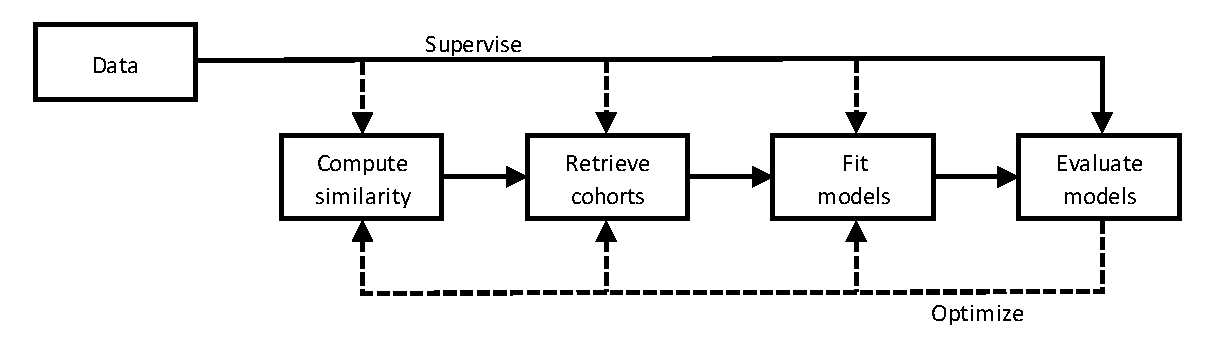
\includegraphics[width=1\linewidth]{Fig5} 

}

\caption{General framework for localized models. Dashed arrows indicate optional steps.}\label{fig:framework}
\end{figure}

Each step can be unsupervised supervised: Unsupervised similarity
measures include discrete measures like the Levenshtein distance and
continuous measures like cosine similarity, while supervised measures
include the Mahalanobis distance and random forest proximity as well as
several composite measures with weights calculated from the data. Most
retrieval steps obtained cohorts with a uniform size (cardinality) or
similarity threshold, and the remaining were likewise only informed by
predictors; thus, while a retrieval step could in principle be
supervised, in this sample none were. Almost all models were supervised,
being that most performed predictive tasks, though Mariuzzi et al.
(1997) modeled only survival rates within localized cohorts. Meanwhile,
each step can be optimized in a ML fashion by having its parameters
tuned to improve performance. We found one study that tuned the
calculation of similarity (Liu et al. 2022), though most uniform cohort
sizes were also tuned. Some earlier studies tuned generalized regression
models, but more recent studies did not.

\small

\begin{longtable}[]{@{}
  >{\raggedright\arraybackslash}p{(\columnwidth - 6\tabcolsep) * \real{0.1928}}
  >{\raggedright\arraybackslash}p{(\columnwidth - 6\tabcolsep) * \real{0.2851}}
  >{\raggedright\arraybackslash}p{(\columnwidth - 6\tabcolsep) * \real{0.1566}}
  >{\raggedright\arraybackslash}p{(\columnwidth - 6\tabcolsep) * \real{0.3655}}@{}}
\caption{\label{tab:framework}Specializations of general framework to
included studies. Flags: R = recurse, S = supervised, T = tuned
(optimized).}\tabularnewline
\toprule\noalign{}
\begin{minipage}[b]{\linewidth}\raggedright
Citation
\end{minipage} & \begin{minipage}[b]{\linewidth}\raggedright
Relevance
\end{minipage} & \begin{minipage}[b]{\linewidth}\raggedright
Retrieval
\end{minipage} & \begin{minipage}[b]{\linewidth}\raggedright
Adaptation
\end{minipage} \\
\midrule\noalign{}
\endfirsthead
\toprule\noalign{}
\begin{minipage}[b]{\linewidth}\raggedright
Citation
\end{minipage} & \begin{minipage}[b]{\linewidth}\raggedright
Relevance
\end{minipage} & \begin{minipage}[b]{\linewidth}\raggedright
Retrieval
\end{minipage} & \begin{minipage}[b]{\linewidth}\raggedright
Adaptation
\end{minipage} \\
\midrule\noalign{}
\endhead
\bottomrule\noalign{}
\endlastfoot
Mariuzzi et al. (1997) & Levenshtein distance\hspace{18em} &
Statistical\hspace{18em} & Survival (S)\hspace{18em} \\
Yearwood and Wilkinson (1997) & Weighted sum (S)\hspace{18em} &
Combinatorial\hspace{18em} & Proportion (S)\hspace{18em} \\
Wyns et al. (2004) & Kohonen mapping\hspace{18em} &
Adaptive\hspace{18em} & Representation (S)\hspace{18em} \\
Park, Kim, and Chun (2006) & Euclidean distance\hspace{18em} &
Statistical (T)\hspace{18em} & Weighted sum (S)\hspace{18em} \\
Elter, Schulz-Wendtland, and Wittenberg (2007) & Entropic
distance\hspace{18em} & Combinatorial\hspace{18em} & Proportion
(S)\hspace{18em} \\
Xu et al. (2008) & Euclidean distance\hspace{18em} &
Combinatorial\hspace{18em} & Proportion (S)\hspace{18em} \\
Song and Kasabov (2006); Kasabov and Hu (2010); Liang, Hu, and Kasabov
(2015); Verma et al. (2015) & Feature selection (R,S)\hspace{18em} &
Combinatorial (R)\hspace{18em} & Fuzzy rules (S,T)\hspace{18em} \\
López et al. (2011) & User-defined\hspace{18em} &
User-defined\hspace{18em} & User-defined\hspace{18em} \\
Lowsky et al. (2013) & Mahalanobis distance (S)\hspace{18em} &
Combinatorial (T)\hspace{18em} & Proportional hazards
(S)\hspace{18em} \\
Campillo-Gimenez et al. (2013) & Weighted overlap\hspace{18em} &
Combinatorial (T)\hspace{18em} & Weighted sum (S)\hspace{18em} \\
Nicolas et al. (2014) & Distance metric learning (S)\hspace{18em} &
Combinatorial\hspace{18em} & Association rules (S,T)\hspace{18em} \\
Ng et al. (2015) & Locally supervised metric learning (S); Feature
selection\hspace{18em} & Combinatorial\hspace{18em} & Logistic model
(S)\hspace{18em} \\
Lee, Maslove, and Dubin (2015) & Cosine similarity\hspace{18em} &
Combinatorial (T)\hspace{18em} & Logistic model (S); Decision tree
(S)\hspace{18em} \\
Vilhena et al. (2016) & Range overlap\hspace{18em} & Clustering
(S)\hspace{18em} & Artificial neural network (S)\hspace{18em} \\
Lee (2017) & Cosine similarity; Random forest proximity (S)\hspace{18em}
& Combinatorial (T)\hspace{18em} & Logistic model (S); Decision tree
(S); Random forest (S)\hspace{18em} \\
Malykh and Rudetskiy (2018) & Unclear\hspace{18em} &
Unclear\hspace{18em} & Unclear\hspace{18em} \\
Zhang et al. (2018) & Gaussian process model\hspace{18em} &
Complete\hspace{18em} & Weighted support vector machine (S); Weighted
Gaussian process regression (S)\hspace{18em} \\
N. Wang et al. (2019) & Weighted sum\hspace{18em} & Combinatorial
(T)\hspace{18em} & Logistic model (S); Random forest (S); Nearest
neighbors (S)\hspace{18em} \\
Ma et al. (2020) & Weighted sum\hspace{18em} &
Combinatorial\hspace{18em} & Extreme learning machine
(S)\hspace{18em} \\
Y. Wang et al. (2020) & Weighted sum\hspace{18em} &
Statistical\hspace{18em} & Linear model\hspace{18em} \\
Tang et al. (2021); Ng et al. (2021) & Locally supervised metric
learning (S)\hspace{18em} & Causal inference matching\hspace{18em} &
Statistical test (S)\hspace{18em} \\
Doborjeh et al. (2022) & Euclidean distance; Signal-to-noise ratio
(S)\hspace{18em} & Statistical (T)\hspace{18em} & Spiking neural network
(S)\hspace{18em} \\
Liu et al. (2022) & Weighted Manhattan distance (R,T)\hspace{18em} &
Proportional (T)\hspace{18em} & Logistic model (S)\hspace{18em} \\
\end{longtable}

\normalsize

\hypertarget{directions-and-expectations-for-future-work}{%
\subsection{Directions and expectations for future
work}\label{directions-and-expectations-for-future-work}}

\hypertarget{performance}{%
\subsubsection{Performance}\label{performance}}

As discussed in Section \ref{rationales}, most studies were premised on
the potential predictive value of localized models. As cautioned in
Section \ref{evaluations}, not all experiments affirmed this premise.
Most of those that did involved using metric learning to improve
retrieval and sometimes iterative optimization of the metric and of the
localized model. Some studies showcased results using a variety of such
specializations (Campillo-Gimenez et al. 2013; Ng et al. 2015; Zhang et
al. 2018; Liu et al. 2022). However, because these advanced
implementations were mostly compared against their precursors or
commonplace alternatives, we cannot speak to their performance or any
trade-offs with respect to each other. This would be a worthy goal of
future work.

The value of this work would be enhanced by standardization and
modularization. First, studies using localized models should locate the
proposed approach and any variations in a shared specification space.
For this purpose, we propose the framework outlined above, at least as a
starting point. When a specification invokes complex techniques, for
example supervised DML or neural network classifiers, it should be
compared at least to alternative specifications using simpler
alternatives. Campillo-Gimenez et al. (2013) and Liu et al. (2022)
provide excellent examples in which all possible choices are toggled and
yield a neatly nested comparison. Additionally, some state-of-the-art
models, including others that obtain individualized predictions, should
be included in comparisons. Finally, implementations should be not only
published on public repositories but designed in such a way that users
familiar with the underlying language can substitute a technique of
their choosing for any part of the specification (similarity, retrieval,
fitting, evaluation). We believe these principles will make reported
results clearer and reproduction and extension easier.

\hypertarget{interpretability}{%
\subsubsection{Interpretability}\label{interpretability}}

While most studies identified outstanding technical needs (Section
\ref{identified-needs}), few emphasized the need to assess human-focused
qualities like user interface and user experience, interpretability,
meaningfulness, or trust. Most studies identified interpretability as an
advantage of localized models, though none evaluated model
interpretability and few proposed new interpretative uses. Lack of trust
in ML tools is a long-recognized problem that direct intepretability of
model components could help alleviate, but this is more often assumed
than demonstrated.

One valuable direction for future work would be to measure the utility
of interpretable components in research and in clinical practice and the
correctness and confidence of users in their interpretations. This is a
necessary precondition for practical use but would also be a valuable
contribution to the experimental literature. Another would be to compare
the localized predictor importance measures obtained from localized
models to the local importance measures used to explain predictions made
by opaque models. This would test both measures for concurrent validity,
while differences between them would inform what settings or cases are
poorly served by one or the other.

\hypertarget{feasibility}{%
\subsubsection{Feasibility}\label{feasibility}}

Much of the reviewed work was motivated by the need for modeling
paradigms that perform well on a variety of tasks and in a variety of
settings. This need demands not only methodologies but also
architectures that are robust, versatile, and compliant in the face of
diverse data models and use restrictions, yet no studies in our sample
addressed the challenges of system interoperability and regulatory
requirements head-on.

CBR and, by extension, localized modeling are especially susceptible to
these challenges, as corpora of past cases must be aggregated from
multiple institutions and from multiple systems within institutions, and
models built on them must then be applicable to out-of-box data
structures as well. Individual systems exhibit many dimensions of
incompleteness (Weiskopf et al. 2013) and vary along other dimensions of
quality (Kohane et al. 2021), and their aggregation for modeling
purposes depends on several kinds of interoperability (Weber 2015).
Successful deployment also depends on satisfying regulatory regimes
designed to protect the privacy of patients, the security of
communications, and trust between parties (Haendel et al. 2021). While
most studies in our sample focused on improving care, increasingly many
over time focused on generalizable knowledge. Therefore, as studies
using localized modeling shift from proof of concept to feasibility,
they will also need to demonstrate practical and regulatory feasibility.

\hypertarget{customizability}{%
\subsubsection{Customizability}\label{customizability}}

The primary goal of these studies was to establish that localized
models, and certain strategies within this paradigm, perform at or above
the level of other predictive models or strategies. From a functionalist
approach to reproducibility (Matarese 2022), then, later studies were
broadly successful at reproducing earlier studies, and later studies
provide sufficient detail to support ongoing reproduction
efforts---though these might be limited by the lack of open-source code
or public implementations. However, the immediate goal of most studes
was to improve care, and an implied need, often enjoined but neither
obtained nor reproduced, was a demonstration of practical use.

We posit that an essential component of practical usefulness is the
ability of the user community to exert some control over the models.
Given the impact on performance of the choice or optimization of the
similarity measure, an important target for user input would be the
importance of certain variables in the calculation of similarity, with
an understanding of how it can impact not only the performance of the
predictions but also the cohort retrieved for the model. For one
example, a user may want to minimize the weight of rare diseases in
medical history in order to retrieve a population with more such cases
in order to better measure their associated risk to the outcome. In
contrast, they may want to increase the weight of the indicating
diagnosis in order to allow fewer patients from similar but distinct
populations to influence the model. For another example, a user may want
to down-weight socioeconomic variables like race--ethnicity in order to
ensure a more diverse modeling cohort. López et al. (2011) took an
important step in this direction with an adjustable and adaptable
implementation. Future purely quantitative work could assess whether
similarity-tuning can achieve these ends more flexibly than strict
inclusion/exclusion criteria.

\hypertarget{conclusions}{%
\subsection{Conclusions}\label{conclusions}}

We propose the term \emph{localized modeling} to encompass an approach
derived from CBR in which parameterized models are fitted in a
standardized way to nearest neighborhoods of past or training cases
according to a measure of patient similarity. We conducted a systematic
search for studies that apply localized models to tasks involving health
data and synthesized these largely independently developed approaches
into a general framework. While the search was limited by low
inter-rater reliability and failure to recover several motivating
examples, the included studies used many of the same underlying tools to
build, optimize, and evaluate their methods. We therefore believe that
our framework can serve to taxonomize ongoing work of this type and
inform the development of customizable implementations. Indeed, the
availability of increasing computational power, the diversity of tasks
to which these models were applied and of technical specifications they
employed, and the apparent lack of any multi-group research program to
date suggest great potential for growth. Whereas precious few of the
reviewed studies used these models for any task other than prediction,
despite widespread suspicion among clinicians of ``black-box'' models
and growing interest in interpretable alternatives, we recommend that
future work put greater emphasis on the development and validation of
interpretable localized models and on their reception by communities of
medical research and clinical practice.

\pagebreak

\hypertarget{appendix}{%
\section*{Appendix}\label{appendix}}
\addcontentsline{toc}{section}{Appendix}

\hypertarget{research-question}{%
\subsection*{Research question}\label{research-question}}
\addcontentsline{toc}{subsection}{Research question}

How is patient similarity--based individualized modeling conducted using
retrospective data?

\hypertarget{purpose-of-review}{%
\subsection*{Purpose of review}\label{purpose-of-review}}
\addcontentsline{toc}{subsection}{Purpose of review}

\begin{enumerate}
\def\labelenumi{\arabic{enumi}.}
\tightlist
\item
  Provide a summary of individualized models to date.
\item
  Lay the groundwork for conducting a comparison study of individualized
  models.
\item
  Provide a framework for future individualized modeling studies.
\end{enumerate}

\hypertarget{search-design}{%
\subsection*{Search design}\label{search-design}}
\addcontentsline{toc}{subsection}{Search design}

The procedure for formulating the search began with an evaluation of the
research question. We highlighted specific elements within our topic of
interest that we found critical to our search and listed them using an
OR of ANDs, pairing terms we believed would provide our desired result.
Following the solidification of the search, a thesaurus was created in
which each term was expanded by synonyms that are similar enough to our
core term to be applicable to our search. The expanded search string was
then evaluated using the PubMed Advanced Search platform. We initially
included each term and their synonyms separately to evaluate what
resulted. Several terms were eliminated due to PubMed classifying them
as ``phrases not found'' and other terms were removed to reduce the
number of results, providing a more concise list of results. At the
conclusions of this process for each individual term, we combined each
search term using an OR of ANDs to ultimately form our search.

The search will have been designed to recover studies of the kind
reviewed by the review papers from which we obtained our ``seed set''.
To validate the final search design, we will determine how many of the
papers in this seed set that are indexed by PubMed are actually
recovered by our search. In most cases, the focus of a review paper is
different from ours, so we will only perform this validation test on the
seed set obtained from two review papers that are (a) closest in focus
to ours and (b) use terminology associated with the two distinct
sub-literatures relevant to our focus: Choudhury \& Begum (2016), which
focuses on case-based reasoning in medicine, and Sharafoddini, Dubin, \&
Lee (2017), which focuses on patient similarity--based prediction models
on health data. The proportion of each PubMed-indexed seed set that is
recovered from our PubMed search provides a rough and optimistic yet
useful estimate of the proportion of the relevant literature that our
full search strategy will recover.

Once we have finalized the search as a logical pattern, we will take the
following steps to generate the sample/corpus of literature that will be
the starting point for our selection process.

\begin{enumerate}
\def\labelenumi{\arabic{enumi}.}
\tightlist
\item
  The logical pattern will be converted to a search string using the
  syntax appropriate to each database in our search strategy. These
  include PubMed (already done as part of the search design), Web of
  Science, Academic Search Premier/Elite, and Mathematical Reviews.
\item
  The search will be conducted on each database and the results
  organized into a Zotero collection, with one subcollection for each
  database.
\item
  Duplicate results will be identified and merged. (A result obtained
  from multiple databases should have only one Zotero entry but should
  be filed under the subcollection for each database in which it was
  found.)
\end{enumerate}

Following discussion among AC, PMJ, and JCB, we discarded results from
Google Scholar due to missing abstracts, missing URLs, high overlap with
other search results, and irreproducibility of the search process.

\hypertarget{search-strings}{%
\subsubsection*{Search strings}\label{search-strings}}
\addcontentsline{toc}{subsubsection}{Search strings}

Here we reproduce the search strings and platform specifications used in
our literature search. We first finalized the \textbf{PubMed} search
string below:\footnote{\url{https://pubmed.ncbi.nlm.nih.gov/?term=(+"case-based+reasoning"+[All+Fields]+OR+"case-based+system"+[All+Fields]+)+OR+(+"individualized+modeling"+[All+Fields]+OR+"personalized+modeling"+[All+Fields]+OR+"customized+modeling"+[All+Fields]+)+OR+(+"individualized+cohort"+[All+Fields]+)+OR+(+(+"patient+similarity"+[All+Fields]+OR+"patient+distance"+[All+Fields]+OR+"patient+connection"+[All+Fields]+OR+"patient+affinity"+[All+Fields]+OR+"patient+clustering"+[All+Fields]+)+AND+(+"cohort+study"+[All+Fields]+)+)&sort=date}}

\begin{verbatim}
(
  "case-based reasoning" [All Fields] OR
  "case-based system" [All Fields]
) OR (
  "individualized modeling" [All Fields] OR
  "personalized modeling" [All Fields] OR
  "customized modeling" [All Fields]
) OR (
  "individualized cohort" [All Fields]
) OR (
  (
    "patient similarity" [All Fields] OR
    "patient distance" [All Fields] OR
    "patient connection" [All Fields] OR
    "patient affinity" [All Fields] OR
    "patient clustering" [All Fields]
  ) AND (
    "cohort study" [All Fields]
  )
)
\end{verbatim}

This search yielded 423 results.

We then generated analogous search strings or search strategies for the
Web of Science, Academic Search Premier, and MathSciNet platforms, based
on the logics and syntaxes of their respective interfaces.

For \textbf{Web of Science}, we searched for several separate
disjunctions derived from the PubMed search string. The separate search
strings and the number of results obtained using each are below.

\begin{longtable}[]{@{}
  >{\raggedright\arraybackslash}p{(\columnwidth - 2\tabcolsep) * \real{0.4444}}
  >{\raggedleft\arraybackslash}p{(\columnwidth - 2\tabcolsep) * \real{0.2361}}@{}}
\toprule\noalign{}
\begin{minipage}[b]{\linewidth}\raggedright
Search string
\end{minipage} & \begin{minipage}[b]{\linewidth}\raggedleft
Number of items
\end{minipage} \\
\midrule\noalign{}
\endhead
\bottomrule\noalign{}
\endlastfoot
\texttt{"case-based\ reasoning"\ OR} \texttt{"case-based\ system"} &
3,636 \\
\texttt{"individualized\ model"\ OR}
\texttt{"individualized\ modeling"\ OR}
\texttt{"personalized\ model"\ OR} \texttt{"personalized\ modeling"\ OR}
\texttt{"customized\ model"} \texttt{"customized\ modeling"} & 444 \\
\texttt{"individualized\ cohort"} & 1 \\
\texttt{"patient\ similarity"\ OR} \texttt{"patient\ distance"\ OR}
\texttt{"patient\ connection"\ OR} \texttt{"patient\ affinity"\ OR}
\texttt{"patient\ clustering"}; Refined search: \texttt{"cohort"} &
48 \\
\end{longtable}

We found the results of the first search string to be predominantly
irrelevant. To reduce review time, these were dropped. The last search
was refined with an additional term following the initial disjunctive
search. Our searches on Web of Science thus yielded 493 results.

When searching \textbf{Academic Search Premier}, we checked the option
``Scholarly (Peer-Reviewed) Journals'', unchecked the option ``Apply
equivalent subjects'', and searched for several separate disjunctions
and conjunctions of strings in the ``TX All Text'' field. We obtained
the resulting citations via email in RIS format.

\begin{longtable}[]{@{}
  >{\raggedright\arraybackslash}p{(\columnwidth - 2\tabcolsep) * \real{0.4444}}
  >{\raggedleft\arraybackslash}p{(\columnwidth - 2\tabcolsep) * \real{0.2361}}@{}}
\toprule\noalign{}
\begin{minipage}[b]{\linewidth}\raggedright
Search string
\end{minipage} & \begin{minipage}[b]{\linewidth}\raggedleft
Number of items
\end{minipage} \\
\midrule\noalign{}
\endhead
\bottomrule\noalign{}
\endlastfoot
\texttt{"case-based\ reasoning"\ OR} \texttt{"case-based\ system"} &
3,283 \\
\texttt{"individualized\ modeling"\ OR}
\texttt{"personalized\ modeling"\ OR} \texttt{"customized\ modeling"} &
100 \\
\texttt{"individualized\ cohort"} & 2 \\
\texttt{"patient\ similarity"\ AND} \texttt{"cohort\ study"} & 14 \\
\texttt{"patient\ distance"\ AND} \texttt{"cohort\ study"} & 15 \\
\texttt{"patient\ connection"\ AND} \texttt{"cohort\ study"} & 6 \\
\texttt{"patient\ affinity"\ AND} \texttt{"cohort\ study"} & 0 \\
\texttt{"patient\ clustering"\ AND} \texttt{"cohort\ study"} & 50 \\
\end{longtable}

We found the results of the first search string to be predominantly
irrelevant. To reduce review time, these were dropped. Our searches on
Academic Search Premier thus yielded 187 results.

For \textbf{MathSciNet}, the portal to the \emph{Mathematical Reviews}
database, we used the same separate searches as for Web of Science, in
some cases expanded to obtain more results. Those which yielded nonzero
numbers of results are below:

\begin{longtable}[]{@{}
  >{\raggedright\arraybackslash}p{(\columnwidth - 2\tabcolsep) * \real{0.4444}}
  >{\raggedleft\arraybackslash}p{(\columnwidth - 2\tabcolsep) * \real{0.2361}}@{}}
\toprule\noalign{}
\begin{minipage}[b]{\linewidth}\raggedright
Search string
\end{minipage} & \begin{minipage}[b]{\linewidth}\raggedleft
Number of items
\end{minipage} \\
\midrule\noalign{}
\endhead
\bottomrule\noalign{}
\endlastfoot
\texttt{"case-based\ reasoning"} & 110 \\
\texttt{"individualized\ model} & 2 \\
\texttt{"patient\ similarity"\ AND} \texttt{"cohort"} & 1 \\
\end{longtable}

Our searches of \emph{Mathematical Reviews} therefore yielded 113
results.

These totaled 1,422 sources from all platforms. We organized the full
results in a public Zotero collection alongside the seed set and created
a single folder for the 25 results reviewed in detail.

\hypertarget{screening-process}{%
\subsection*{Screening process}\label{screening-process}}
\addcontentsline{toc}{subsection}{Screening process}

Most deduplication was done automatically in Covidence. As full-text
review was done in Zotero, some additional duplicates were noticed and
merged.

When abstracts were not obtained by search or by Covidence, we attempted
to find them online using DOIs; when an abstract could not be found,
screening was based on the title alone. We decided to screen titles and
abstracts conservatively, rejecting only studies that were clearly
outside the scope of our review. The reasons for rejection were four, as
discussed in the main text: a. Exclude non clinical/non medical setting
b. Must be in English c.~Must be original study (not reviews, surveys,
opinion, news) d.~Exclude if search term clearly has different meaning
than intended (Two examples of (d) are the use of the term
``personalized model'' to refer in some cases to parameterized models
tuned to individual patient measurements and in others to
patient-centered models of care.) Studies that passed title/abstract
screen were exported to Zotero.

\hypertarget{selection-process}{%
\subsection*{Selection process}\label{selection-process}}
\addcontentsline{toc}{subsection}{Selection process}

Some PDFs were obtained using Zotero from a university workstation, and
the remaining were obtained through university library services. The
review process is detailed in Section \ref{full-text-review}.

Our selection of relevant papers from the search corpus was based on the
following inclusion/exclusion criteria:

\begin{itemize}
\tightlist
\item
  Uses labeled case-level (empirical) data set
\item
  Defines a continuous-valued multivariate case similarity measure
\item
  Uses the similarity measure to select cohorts for index cases from the
  corpus
\item
  Fits statistical models to cohorts to make inferences about index
  cases
\end{itemize}

We decided after concluding full-text review to perform one round of
citation-tracking, of citations within the Methods (or analogous)
sections of the included entries.

\hypertarget{update}{%
\subsection*{Update}\label{update}}
\addcontentsline{toc}{subsection}{Update}

Of the 25 studies included, 4 showed up in no database searches (but
included from the seed set), 1 was obtained via reference tracking, and,
of the remaining 20 found through the database searches, only 1 was not
found in PubMed or Web of Science. That one was instead found in
Mathematical Reviews. Since MR returns about the same volume of results
as WoS and PM, we omitted it from the update.

We applied the search terms exactly as before but restricted the dates
to 2021 July 19 (the beginning of the date range for our original
searches) or later. We omitted the WoS search that returned
impractically many results the first time around and was omitted then.

We ran the update search on 2024 January 24.

The PubMed update returned 97 results. The Web of Science refresher
returned 272 + 0 + 26 = 298 results. Covidence removed duplicates, so
that 348 studies were slated for screening.

Screening by title and abstract was done in two waves. First, PM
excluded only on account of a study not being (a) clinical/medical, (b)
English, and (c) original. Then, JCB then excluded on account of a study
being (d) indicated by the intended meanings of our search terms.

\hypertarget{analysis-and-synthesis}{%
\subsection*{Analysis and synthesis}\label{analysis-and-synthesis}}
\addcontentsline{toc}{subsection}{Analysis and synthesis}

Because we could not predict the scope of methodological approaches we
would encounter, we did not prepare specific analyses or syntheses
\emph{a priori}.

\hypertarget{methodological-elements}{%
\subsection*{Methodological elements}\label{methodological-elements}}
\addcontentsline{toc}{subsection}{Methodological elements}

Table \ref{tab:composite} and Figure \ref{fig:methods} summarize the
techniques and terminology used by the included studies, as referred to
in the main text.

\small

\begin{longtable}[]{@{}
  >{\raggedright\arraybackslash}p{(\columnwidth - 4\tabcolsep) * \real{0.1082}}
  >{\raggedright\arraybackslash}p{(\columnwidth - 4\tabcolsep) * \real{0.4433}}
  >{\raggedright\arraybackslash}p{(\columnwidth - 4\tabcolsep) * \real{0.4485}}@{}}
\caption{\label{tab:composite}Methodological elements of studies
included in the synthesis.}\tabularnewline
\toprule\noalign{}
\begin{minipage}[b]{\linewidth}\raggedright
Citation
\end{minipage} & \begin{minipage}[b]{\linewidth}\raggedright
Elements
\end{minipage} & \begin{minipage}[b]{\linewidth}\raggedright
Terminology
\end{minipage} \\
\midrule\noalign{}
\endfirsthead
\toprule\noalign{}
\begin{minipage}[b]{\linewidth}\raggedright
Citation
\end{minipage} & \begin{minipage}[b]{\linewidth}\raggedright
Elements
\end{minipage} & \begin{minipage}[b]{\linewidth}\raggedright
Terminology
\end{minipage} \\
\midrule\noalign{}
\endhead
\bottomrule\noalign{}
\endlastfoot
Yearwood and Wilkinson (1997) & supervised similarity learning & CBR;
case-structured retrieval \\
Mariuzzi et al. (1997) & predictive modeling on similarity cohorts &
CBR; targeted subsampling \\
Wyns et al. (2004) & unsupervised similarity learning & Combined Kohonen
type neural network-case-based reasoning \\
Park, Kim, and Chun (2006) & supervised cohort construction & CBR,
statistical case-based reasoning \\
Song and Kasabov (2006) & supervised similarity learning & Transductive
inference \\
Elter, Schulz-Wendtland, and Wittenberg (2007) & unsupervised similarity
learning & CBR; entropic distance measure \\
Xu et al. (2008) & tiered constraint; similarity matching & CBR \\
López et al. (2011) & interactive implementation & CBR; eXiT*CBR \\
Kasabov and Hu (2010) & predictive modeling on similarity cohorts &
Personalized model \\
Verma et al. (2015) & predictive modeling on similarity cohorts &
Personalized modeling; TWNFI \\
Liang, Hu, and Kasabov (2015) & predictive modeling on similarity
cohorts & Local modeling; personalized modeling; TWNFI \\
Lowsky et al. (2013) & predictive modeling on similarity cohorts &
K-nearest neighbors survival \\
Campillo-Gimenez et al. (2013) & supervised similarity learning & CBR \\
Nicolas et al. (2014) & supervised similarity learning & CBR \\
Ng et al. (2015) & predictive modeling on similarity cohorts;
explanatory modeling on similarity cohorts & Personalized predictive
model \\
Lee, Maslove, and Dubin (2015) & predictive modeling on similarity
cohorts & Personalized prediction \\
Vilhena et al. (2016) & supervised similarity learning; predictive
modeling on similarity cohorts & CBR \\
Lee (2017) & predictive modeling on similarity cohorts &
Patient-specific predictive model \\
Zhang et al. (2018) & whole-population weight learning & Gaussian
processes \\
Malykh and Rudetskiy (2018) & unclear & CBR \\
Ma et al. (2020) & predictive modeling on similarity cohorts &
Personalized model \\
N. Wang et al. (2019) & predictive modeling on similarity cohorts &
Personalized predictive modeling \\
Y. Wang et al. (2020) & descriptive modeling on similarity cohorts &
CBR \\
Liu et al. (2022) & NA & Personalized model with transfer learning \\
Doborjeh et al. (2022) & NA & Personalized spiking neural network \\
Tang et al. (2021); Ng et al. (2021) & supervised similarity learning;
predictive modeling on similarity cohorts & Similarity model,
personalized model, precision cohort, personalized treatment options \\
\end{longtable}

\normalsize

\begin{figure}

{\centering 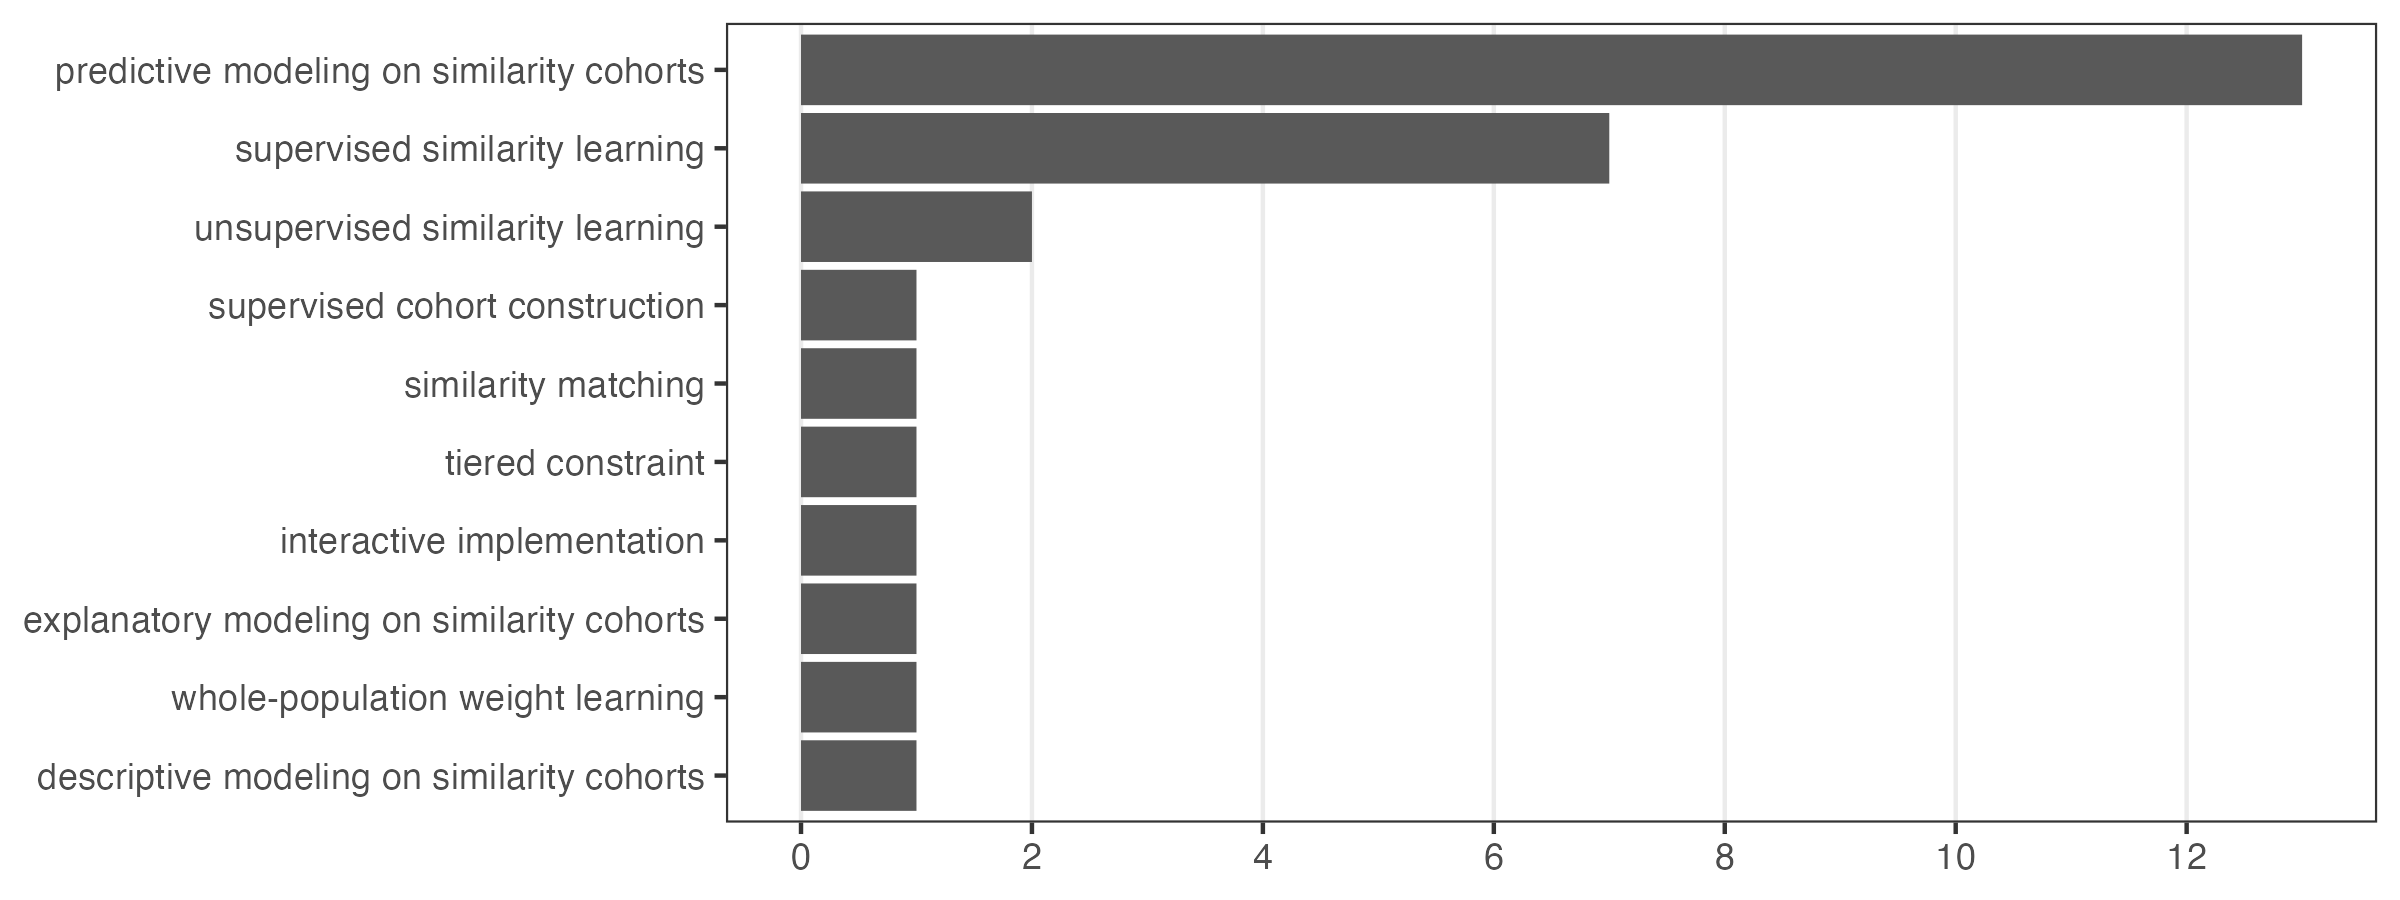
\includegraphics[width=1\linewidth]{Fig4} 

}

\caption{Frequency of recurring methodological elements across included studies.}\label{fig:methods}
\end{figure}

\hypertarget{performance-evaluations-and-comparisons}{%
\subsection*{Performance evaluations and
comparisons}\label{performance-evaluations-and-comparisons}}
\addcontentsline{toc}{subsection}{Performance evaluations and
comparisons}

Table \ref{tab:performance} summarizes the evaluations and comparisons
made of methods proposed in the included studies. In most cases, not all
performance results are included; for the sake of concision, only what
we judged to be the headline results, using the primary evaluation
metrics, are reproduced here. The table contains no original results.

\begin{landscape}

%\textbf{TODO: Place vertical separators between major columns.}

\small

\begin{longtable}[]{@{}
  >{\raggedright\arraybackslash}p{(\columnwidth - 12\tabcolsep) * \real{0.1088}}
  >{\raggedright\arraybackslash}p{(\columnwidth - 12\tabcolsep) * \real{0.0725}}
  >{\raggedright\arraybackslash}p{(\columnwidth - 12\tabcolsep) * \real{0.1658}}
  >{\raggedright\arraybackslash}p{(\columnwidth - 12\tabcolsep) * \real{0.2435}}
  >{\raggedleft\arraybackslash}p{(\columnwidth - 12\tabcolsep) * \real{0.0984}}
  >{\raggedright\arraybackslash}p{(\columnwidth - 12\tabcolsep) * \real{0.2124}}
  >{\raggedleft\arraybackslash}p{(\columnwidth - 12\tabcolsep) * \real{0.0984}}@{}}
\caption{\label{tab:performance}Evaluations of proposed methods and
comparisons to alternative methods. (See original studies for full names
and descriptions.)}\tabularnewline
\toprule\noalign{}
\begin{minipage}[b]{\linewidth}\raggedright
Citation
\end{minipage} & \begin{minipage}[b]{\linewidth}\raggedright
Measure
\end{minipage} & \begin{minipage}[b]{\linewidth}\raggedright
Problem
\end{minipage} & \begin{minipage}[b]{\linewidth}\raggedright
Proposals
\end{minipage} & \begin{minipage}[b]{\linewidth}\raggedleft
\end{minipage} & \begin{minipage}[b]{\linewidth}\raggedright
Comparators
\end{minipage} & \begin{minipage}[b]{\linewidth}\raggedleft
\end{minipage} \\
\midrule\noalign{}
\endfirsthead
\toprule\noalign{}
\begin{minipage}[b]{\linewidth}\raggedright
Citation
\end{minipage} & \begin{minipage}[b]{\linewidth}\raggedright
Measure
\end{minipage} & \begin{minipage}[b]{\linewidth}\raggedright
Problem
\end{minipage} & \begin{minipage}[b]{\linewidth}\raggedright
Proposals
\end{minipage} & \begin{minipage}[b]{\linewidth}\raggedleft
\end{minipage} & \begin{minipage}[b]{\linewidth}\raggedright
Comparators
\end{minipage} & \begin{minipage}[b]{\linewidth}\raggedleft
\end{minipage} \\
\midrule\noalign{}
\endhead
\bottomrule\noalign{}
\endlastfoot
Wyns et al. (2004) & Accuracy & Arthritis & Kohonen + CBR &
75.60\%\hspace{6em} & Kohonen mapping & 54.70\%\hspace{6em} \\
& & & & \hspace{6em} & CBR & 60.40\%\hspace{6em} \\
& & & & \hspace{6em} & Quest & 50.90\%\hspace{6em} \\
& & & & \hspace{6em} & backpropagation & 54.70\%\hspace{6em} \\
\midrule\noalign{}
Park, Kim, and Chun (2006) & Accuracy & Dermatology & Statistical CBR &
96.57\%\hspace{6em} & CBR & 95.43\%\hspace{6em} \\
& & & & \hspace{6em} & C5.0 & 93.71\%\hspace{6em} \\
& & & & \hspace{6em} & CART & 92.00\%\hspace{6em} \\
& & & & \hspace{6em} & LR & 91.14\%\hspace{6em} \\
& & & & \hspace{6em} & NN & 88.29\%\hspace{6em} \\
& & Heart & Statistical CBR & 83.70\%\hspace{6em} & LR &
84.44\%\hspace{6em} \\
& & & & \hspace{6em} & NN & 82.22\%\hspace{6em} \\
& & & & \hspace{6em} & CBR & 81.85\%\hspace{6em} \\
& & & & \hspace{6em} & CART & 76.67\%\hspace{6em} \\
& & & & \hspace{6em} & C5.0 & 76.30\%\hspace{6em} \\
& & Breast & Statistical CBR & 96.96\%\hspace{6em} & NN &
97.50\%\hspace{6em} \\
& & & & \hspace{6em} & CBR & 96.61\%\hspace{6em} \\
& & & & \hspace{6em} & LR & 96.61\%\hspace{6em} \\
& & & & \hspace{6em} & C5.0 & 94.29\%\hspace{6em} \\
& & & & \hspace{6em} & CART & 92.14\%\hspace{6em} \\
& & Diabetes & Statistical CBR & 76.32\%\hspace{6em} & LR &
77.11\%\hspace{6em} \\
& & & & \hspace{6em} & CBR & 73.16\%\hspace{6em} \\
& & & & \hspace{6em} & C5.0 & 73.15\%\hspace{6em} \\
& & & & \hspace{6em} & CART & 72.89\%\hspace{6em} \\
& & & & \hspace{6em} & NN & 65.39\%\hspace{6em} \\
& & Liver & Statistical CBR & 66.76\%\hspace{6em} & CART &
67.94\%\hspace{6em} \\
& & & & \hspace{6em} & LR & 67.35\%\hspace{6em} \\
& & & & \hspace{6em} & C5.0 & 66.47\%\hspace{6em} \\
& & & & \hspace{6em} & CBR & 60.88\%\hspace{6em} \\
& & & & \hspace{6em} & NN & 55.59\%\hspace{6em} \\
\midrule\noalign{}
Song and Kasabov (2006) & RMSE & GFR & TWNFI & 7.08\hspace{6em} & MDRD &
7.74\hspace{6em} \\
& & & & \hspace{6em} & MLP & 8.38\hspace{6em} \\
& & & & \hspace{6em} & ANFIS & 7.40\hspace{6em} \\
& & & & \hspace{6em} & DENFIS & 7.22\hspace{6em} \\
& & & & \hspace{6em} & TNFI & 7.28\hspace{6em} \\
\midrule\noalign{}
Elter, Schulz-Wendtland, and Wittenberg (2007) & AUROC & mammography
mass region & CBR & 0.885\hspace{6em} & DT & 0.872\hspace{6em} \\
& & & & \hspace{6em} & ANN & 0.882\hspace{6em} \\
\midrule\noalign{}
Xu et al. (2008) & Accuracy & Return-to-work & CBR & 62.5\%\hspace{6em}
& LR & 71.2\%\hspace{6em} \\
\midrule\noalign{}
Kasabov and Hu (2010) & Accuracy & Colon cancer diagnosis & TWNFI &
91.9\%\hspace{6em} & MLR (Personalized) & 82.3\%\hspace{6em} \\
& & & & \hspace{6em} & SVM (Personalized) & 90.3\%\hspace{6em} \\
& & & & \hspace{6em} & WKNN & 90.3\%\hspace{6em} \\
& & Crohn's disease risk & TWNFI & 82.45\%\hspace{6em} & &
\hspace{6em} \\
\midrule\noalign{}
Liang, Hu, and Kasabov (2015) & Accuracy & Colon cancer & knnGSA &
85.48\%\hspace{6em} & SVM & 82.14\%\hspace{6em} \\
& & & svmGSA & 87.10\%\hspace{6em} & ECF & 72.30\%\hspace{6em} \\
& & & & \hspace{6em} & KNN & 82.14\%\hspace{6em} \\
& & & & \hspace{6em} & WKNN & 82.14\%\hspace{6em} \\
& & Leukemia & knnGSA & 97.22\%\hspace{6em} & SVM &
95.83\%\hspace{6em} \\
& & & svmGSA & 97.22\%\hspace{6em} & ECF & 94.44\%\hspace{6em} \\
& & & & \hspace{6em} & KNN & 94.44\%\hspace{6em} \\
& & & & \hspace{6em} & WKNN & 94.44\%\hspace{6em} \\
& & Lymphoma & knnGSA & 94.81\%\hspace{6em} & SVM &
93.51\%\hspace{6em} \\
& & & svmGSA & 94.81\%\hspace{6em} & ECF & 92.21\%\hspace{6em} \\
& & & & \hspace{6em} & KNN & 93.51\%\hspace{6em} \\
& & & & \hspace{6em} & WKNN & 93.51\%\hspace{6em} \\
& & Lung cancer & knnGSA & 98.34\%\hspace{6em} & SVM &
95.31\%\hspace{6em} \\
& & & svmGSA & 98.90\%\hspace{6em} & ECF & 92.87\%\hspace{6em} \\
& & & & \hspace{6em} & KNN & 96.60\%\hspace{6em} \\
& & & & \hspace{6em} & WKNN & 95.50\%\hspace{6em} \\
\midrule\noalign{}
Lowsky et al. (2013) & Relative IPEC & Graft survival & MKNN &
0.973\hspace{6em} & RSF & 0.957\hspace{6em} \\
\midrule\noalign{}
Campillo-Gimenez et al. (2013) & AUROC & Waitlist registration, complete
& CBR + Wj & 89.8\%\hspace{6em} & LR & 92.0\%\hspace{6em} \\
& & & CBR + Wk & 90.7\%\hspace{6em} & Standalone CBR &
90.4\%\hspace{6em} \\
& & & CBR + Wj + Wk & 87.4\%\hspace{6em} & & \hspace{6em} \\
& & Waitlist registration, stepwise & CBR + Wj & 82.7\%\hspace{6em} & LR
& 92.1\%\hspace{6em} \\
& & & CBR + Wk & 86.2\%\hspace{6em} & Standalone CBR &
91.4\%\hspace{6em} \\
& & & CBR + Wj + Wk & 88.5\%\hspace{6em} & & \hspace{6em} \\
\midrule\noalign{}
Nicolas et al. (2014) & Accuracy & Nevus & Collaborative + rules &
98\%\hspace{6em} & Dermoscopy CBR & 92\%\hspace{6em} \\
& & & Collaborative + rules + DML & 100\%\hspace{6em} & Confocal CBR &
96\%\hspace{6em} \\
& & & & \hspace{6em} & Collaborative & 95\%\hspace{6em} \\
\midrule\noalign{}
Ng et al. (2015) & AUROC & Diabetes onset & Personalized LR
(LSML+FeatureFiltering) & 0.624\hspace{6em} & KNN & 0.617\hspace{6em} \\
& & & Personalized LR (LSML) & 0.619\hspace{6em} & Global LR &
0.611\hspace{6em} \\
& & & Personalized LR (Euclidean) & 0.614\hspace{6em} & &
\hspace{6em} \\
& & & Personalized LR (Random) & 0.602\hspace{6em} & & \hspace{6em} \\
\midrule\noalign{}
Lee, Maslove, and Dubin (2015) & AUROC & 30-day mortality &
Individualized LR & 0.830\hspace{6em} & Individualized DC &
0.797\hspace{6em} \\
& & & Individualized DT & 0.753\hspace{6em} & & \hspace{6em} \\
\midrule\noalign{}
Lee (2017) & AUROC & & Individualized LR & 0.824\hspace{6em} &
Individualized DC & 0.801\hspace{6em} \\
& & & Individualized DT & 0.779\hspace{6em} & & \hspace{6em} \\
& & & Individualized RF & 0.839\hspace{6em} & & \hspace{6em} \\
& & & Individualized CSRF & 0.832\hspace{6em} & & \hspace{6em} \\
\midrule\noalign{}
Malykh and Rudetskiy (2018) & Accuracy & J13/pneumonia & Case-based NN &
81.6\%\hspace{6em} & & \hspace{6em} \\
& & K80.1/gallbladder & Case-based NN & 76.7\%\hspace{6em} & &
\hspace{6em} \\
& & H25.1/age-related cataract & Case-based NN & 94.9\%\hspace{6em} & &
\hspace{6em} \\
& & H26.2/complicated cataract & Case-based NN & 91.4\%\hspace{6em} & &
\hspace{6em} \\
& & 167.4/encephalopathy & Case-based NN & 72.4\%\hspace{6em} & &
\hspace{6em} \\
& & 167.9/CBD & Case-based NN & 75.4\%\hspace{6em} & & \hspace{6em} \\
& & N20.1/ureter & Case-based NN & 58.7\%\hspace{6em} & &
\hspace{6em} \\
\midrule\noalign{}
Zhang et al. (2018) & AUROC & Cognitive impairment & Gaussian process
regression with custom kernel & 0.92\hspace{6em} & linear regression
without regularization & 0.81\hspace{6em} \\
& & & & \hspace{6em} & LASSO regression & 0.85\hspace{6em} \\
& & & & \hspace{6em} & ridge regression & 0.87\hspace{6em} \\
& & & & \hspace{6em} & RF & 0.90\hspace{6em} \\
& & & & \hspace{6em} & gradient boosting regression tree &
0.91\hspace{6em} \\
& & & & \hspace{6em} & XGBoost & 0.91\hspace{6em} \\
& & & & \hspace{6em} & kernel support vector regressor &
0.92\hspace{6em} \\
& & Parkinson's disease & Gaussian process regression with custom kernel
& 0.875\hspace{6em} & linear regression without regularization &
0.820\hspace{6em} \\
& & & & \hspace{6em} & ridge regression & 0.798\hspace{6em} \\
& & & & \hspace{6em} & RF & 0.734\hspace{6em} \\
& & & & \hspace{6em} & gradient boosting regression tree &
0.825\hspace{6em} \\
& & & & \hspace{6em} & kernel support vector regressor &
0.778\hspace{6em} \\
\midrule\noalign{}
N. Wang et al. (2019) & AUROC & Diabetes & Personalized RF &
0.90\hspace{6em} & & \hspace{6em} \\
& & & Personalized KNN & 0.82\hspace{6em} & & \hspace{6em} \\
& & & Personalized LR & 0.89\hspace{6em} & & \hspace{6em} \\
\midrule\noalign{}
Ma et al. (2020) & AUROC & Discharge at 10 days & One-class JITL-ELM &
0.8510\hspace{6em} & ELM & 0.4973\hspace{6em} \\
& & & & \hspace{6em} & JITL-ELM & 0.2014\hspace{6em} \\
& & & & \hspace{6em} & One-class ELM & 0.7588\hspace{6em} \\
& & & & \hspace{6em} & One-class SVM & 0.4647\hspace{6em} \\
\midrule\noalign{}
Liu et al. (2022) & AUROC & Acute kidney injury & & \hspace{6em} &
Global & 0.684\hspace{6em} \\
& & & & \hspace{6em} & Risk-ranking & 0.708\hspace{6em} \\
& & & & \hspace{6em} & PM-Kmeans & 0.721\hspace{6em} \\
& & & & \hspace{6em} & PM-Kmeans \& TL & 0.759\hspace{6em} \\
& & & & \hspace{6em} & PM-kNN & 0.732\hspace{6em} \\
& & & & \hspace{6em} & PM-kNN \& WS & 0.738\hspace{6em} \\
& & & & \hspace{6em} & PM-kNN \& TL & 0.769\hspace{6em} \\
& & & & \hspace{6em} & PM-kNN \& TL \& WS & 0.771\hspace{6em} \\
& & & & \hspace{6em} & PM-kNN \& WS \& SL & 0.744\hspace{6em} \\
& & & & \hspace{6em} & PMTL & 0.779\hspace{6em} \\
\midrule\noalign{}
Doborjeh et al. (2022) & Accuracy & Stroke & Personalized SNN &
60.70\%\hspace{6em} & & \hspace{6em} \\
\end{longtable}

\normalsize

\end{landscape}

\hypertarget{data-and-code}{%
\subsection{Data and code}\label{data-and-code}}

Search results are publicly available in a Zotero group library. Data
collected or encoded for included studies are publicly available in two
Google Sheets. Code used to analyze these data and generate this
manuscript is publicly available in a GitHub repository.

\begin{itemize}
\tightlist
\item
  Search results, included studies, and other bibliography:
  \url{https://www.zotero.org/groups/5017571/imsr/}
\item
  Bibliographic and methodological properties of included studies:
  \url{https://docs.google.com/spreadsheets/d/1tpWMhYH2pyRT55K7n2J2XFs-kEV_JTuCDmXzJ4BBgNo/}
\item
  Terminology and composite techniques of included studies:
  \url{https://docs.google.com/spreadsheets/d/1xvDJwiLBoI2oz8fxHJ5MjNmiju_RAlK7RJv-wXe1DAs/}
\item
  Code used to conduct analyses and prepare the manuscript:
  \url{https://github.com/corybrunson/imsr}
\end{itemize}

\hypertarget{references}{%
\section*{References}\label{references}}
\addcontentsline{toc}{section}{References}

\hypertarget{refs}{}
\begin{CSLReferences}{1}{0}
\leavevmode\vadjust pre{\hypertarget{ref-Aamodt1994}{}}%
Aamodt, Agnar, and Enric Plaza. 1994. {``Case-{Based Reasoning}:
{Foundational Issues}, {Methodological Variations}, and {System
Approaches}.''} \emph{AI Communications} 7 (1): 39--59.
\url{https://doi.org/10.3233/AIC-1994-7104}.

\leavevmode\vadjust pre{\hypertarget{ref-Begum2011}{}}%
Begum, Shahina, Mobyen Uddin Ahmed, Peter Funk, Ning Xiong, and Mia
Folke. 2011. {``Case-{Based Reasoning Systems} in the {Health Sciences}:
{A Survey} of {Recent Trends} and {Developments}.''} \emph{IEEE
Transactions on Systems, Man, and Cybernetics, Part C (Applications and
Reviews)} 41 (4): 421--34.
\url{https://doi.org/10.1109/TSMCC.2010.2071862}.

\leavevmode\vadjust pre{\hypertarget{ref-Bellet2014}{}}%
Bellet, Aurélien, Amaury Habrard, and Marc Sebban. 2014. {``A {Survey}
on {Metric Learning} for {Feature Vectors} and {Structured Data}.''}
arXiv. \url{https://doi.org/10.48550/arXiv.1306.6709}.

\leavevmode\vadjust pre{\hypertarget{ref-Biecek2021}{}}%
Biecek, Przemyslaw, and Tomasz Burzykowski. 2021. \emph{Explanatory
{Model Analysis}: {Explore}, {Explain}, and {Examine Predictive
Models}}. New York: {Chapman and Hall/CRC}.

\leavevmode\vadjust pre{\hypertarget{ref-Brauneck2023}{}}%
Brauneck, Alissa, Louisa Schmalhorst, Mohammad Mahdi Kazemi Majdabadi,
Mohammad Bakhtiari, Uwe Völker, Jan Baumbach, Linda Baumbach, and
Gabriele Buchholtz. 2023. {``Federated {Machine Learning},
{Privacy-Enhancing Technologies}, and {Data Protection Laws} in {Medical
Research}: {Scoping Review}.''} \emph{Journal of Medical Internet
Research} 25 (1): e41588. \url{https://doi.org/10.2196/41588}.

\leavevmode\vadjust pre{\hypertarget{ref-CampilloGimenez2013}{}}%
Campillo-Gimenez, Boris, Wassim Jouini, Sahar Bayat, and Marc Cuggia.
2013. {``Improving {Case-Based Reasoning Systems} by {Combining
K-Nearest Neighbour Algorithm} with {Logistic Regression} in the
{Prediction} of {Patients}' {Registration} on the {Renal Transplant
Waiting List}.''} Edited by Randen Lee Patterson. \emph{PLOS ONE} 8 (9):
e71991. \url{https://doi.org/10.1371/journal.pone.0071991}.

\leavevmode\vadjust pre{\hypertarget{ref-Choudhury2016}{}}%
Choudhury, Nabanita, and Shahin Ara Begum. 2016. {``A {Survey} on
{Case-based Reasoning} in {Medicine}.''} \emph{International Journal of
Advanced Computer Science and Applications} 7 (8).
\url{https://doi.org/10.14569/IJACSA.2016.070820}.

\leavevmode\vadjust pre{\hypertarget{ref-Dai2020}{}}%
Dai, Leyu, He Zhu, and Dianbo Liu. 2020. {``Patient Similarity: Methods
and Applications.''} \emph{arXiv:2012.01976 {[}Cs{]}}, December.
\url{https://arxiv.org/abs/2012.01976}.

\leavevmode\vadjust pre{\hypertarget{ref-Doborjeh2022}{}}%
Doborjeh, Maryam, Zohreh Doborjeh, Alexander Merkin, Rita Krishnamurthi,
Reza Enayatollahi, Valery Feigin, and Nikola Kasabov. 2022.
{``Personalized {Spiking Neural Network Models} of {Clinical} and
{Environmental Factors} to {Predict Stroke}.''} \emph{Cognitive
Computation} 14 (6): 2187--2202.
\url{https://doi.org/10.1007/s12559-021-09975-x}.

\leavevmode\vadjust pre{\hypertarget{ref-Doyle2006}{}}%
Doyle, Dónal, Pádraig Cunningham, and Paul Walsh. 2006. {``An Evaluation
of the Usefulness of Explanation in a Case-Based Reasoning System for
Decision Support in Bronchiolitis Treatment.''} \emph{Computational
Intelligence} 22 (3-4): 269--81.
\url{https://doi.org/10.1111/j.1467-8640.2006.00288.x}.

\leavevmode\vadjust pre{\hypertarget{ref-Elter2007}{}}%
Elter, M., R. Schulz-Wendtland, and T. Wittenberg. 2007. {``The
Prediction of Breast Cancer Biopsy Outcomes Using Two {CAD} Approaches
That Both Emphasize an Intelligible Decision Process.''} \emph{Medical
Physics} 34 (11): 4164--72. \url{https://doi.org/10.1118/1.2786864}.

\leavevmode\vadjust pre{\hypertarget{ref-Fang2021}{}}%
Fang, Hao Sen Andrew, Ngiap Chuan Tan, Wei Ying Tan, Ronald Wihal Oei,
Mong Li Lee, and Wynne Hsu. 2021. {``Patient Similarity Analytics for
Explainable Clinical Risk Prediction.''} \emph{BMC Medical Informatics
\& Decision Making} 21 (1): 1--12.

\leavevmode\vadjust pre{\hypertarget{ref-Gierl1998}{}}%
Gierl, Lothar, Mathias Bull, and Rainer Schmidt. 1998. {``{CBR} in
{Medicine}.''} In \emph{Case-{Based Reasoning Technology}}, edited by
Mario Lenz, Hans-Dieter Burkhard, Brigitte Bartsch-Spörl, and Stefan
Wess, 1400:273--97. Berlin, Heidelberg: Springer Berlin Heidelberg.
\url{https://doi.org/10.1007/3-540-69351-3_11}.

\leavevmode\vadjust pre{\hypertarget{ref-Goyal2008}{}}%
Goyal, Navin, Yury Lifshits, and Hinrich Schütze. 2008. {``Disorder
Inequality: A Combinatorial Approach to Nearest Neighbor Search.''} In
\emph{Proceedings of the 2008 {International Conference} on {Web Search}
and {Data Mining}}, 25--32. {WSDM} '08. New York, NY, USA: Association
for Computing Machinery. \url{https://doi.org/10.1145/1341531.1341538}.

\leavevmode\vadjust pre{\hypertarget{ref-Haendel2021}{}}%
Haendel, Melissa A, Christopher G Chute, Tellen D Bennett, David A
Eichmann, Justin Guinney, Warren A Kibbe, Philip R O Payne, et al. 2021.
{``The {National COVID Cohort Collaborative} ({N3C}): {Rationale},
Design, Infrastructure, and Deployment.''} \emph{Journal of the American
Medical Informatics Association} 28 (3): 427--43.
\url{https://doi.org/10.1093/jamia/ocaa196}.

\leavevmode\vadjust pre{\hypertarget{ref-Kasabov2010}{}}%
Kasabov, Nikola, and Yingjie Hu. 2010. {``Integrated Optimisation Method
for Personalised Modelling and Case Studies for Medical Decision
Support.''} \emph{International Journal of Functional Informatics and
Personalised Medicine} 3 (3): 236--56.
\url{https://doi.org/10.1504/IJFIPM.2010.039123}.

\leavevmode\vadjust pre{\hypertarget{ref-Kohane2021}{}}%
Kohane, Isaac S., Bruce J. Aronow, Paul Avillach, Brett K.
Beaulieu-Jones, Riccardo Bellazzi, Robert L. Bradford, Gabriel A. Brat,
et al. 2021. {``What {Every Reader Should Know About Studies Using
Electronic Health Record Data} but {May Be Afraid} to {Ask}.''}
\emph{Journal of Medical Internet Research} 23 (3): e22219.
\url{https://doi.org/10.2196/22219}.

\leavevmode\vadjust pre{\hypertarget{ref-Kolodner1992}{}}%
Kolodner, Janet L. 1992. {``An Introduction to Case-Based Reasoning.''}
\emph{Artificial Intelligence Review} 6 (1): 3--34.
\url{https://doi.org/10.1007/BF00155578}.

\leavevmode\vadjust pre{\hypertarget{ref-Lee2017}{}}%
Lee, Joon. 2017. {``Patient-{Specific Predictive Modeling Using Random
Forests}: {An Observational Study} for the {Critically Ill}.''}
\emph{JMIR Medical Informatics} 5 (1): e3.
\url{https://doi.org/10.2196/medinform.6690}.

\leavevmode\vadjust pre{\hypertarget{ref-Lee2015}{}}%
Lee, Joon, David M. Maslove, and Joel A. Dubin. 2015. {``Personalized
{Mortality Prediction Driven} by {Electronic Medical Data} and a
{Patient Similarity Metric}.''} Edited by Frank Emmert-Streib.
\emph{PLOS ONE} 10 (5): e0127428.
\url{https://doi.org/10.1371/journal.pone.0127428}.

\leavevmode\vadjust pre{\hypertarget{ref-Liang2015}{}}%
Liang, W, YJ Hu, and N Kasabov. 2015. {``Evolving Personalized Modeling
System for Integrated Feature, Neighborhood and Parameter Optimization
Utilizing Gravitational Search Algorithm.''} \emph{Evolving Systems} 6
(1): 1--14. \url{https://doi.org/10.1007/s12530-013-9081-x}.

\leavevmode\vadjust pre{\hypertarget{ref-Liu2022}{}}%
Liu, Kang, Xiangzhou Zhang, Weiqi Chen, Alan S. L. Yu, John A. Kellum,
Michael E. Matheny, Steven Q. Simpson, Yong Hu, and Mei Liu. 2022.
{``Development and {Validation} of a {Personalized Model With Transfer
Learning} for {Acute Kidney Injury Risk Estimation Using Electronic
Health Records}.''} \emph{JAMA Network Open} 5 (7): e2219776.
\url{https://doi.org/10.1001/jamanetworkopen.2022.19776}.

\leavevmode\vadjust pre{\hypertarget{ref-Longhurst2014}{}}%
Longhurst, Christopher A., Robert A. Harrington, and Nigam H. Shah.
2014. {``A {`{Green Button}'} {For Using Aggregate Patient Data At The
Point Of Care}.''} \emph{Health Affairs} 33 (7): 1229--35.
\url{https://doi.org/10.1377/hlthaff.2014.0099}.

\leavevmode\vadjust pre{\hypertarget{ref-Lopez2011}{}}%
López, Beatriz, Carles Pous, Pablo Gay, Albert Pla, Judith Sanz, and
Joan Brunet. 2011. {``{eXiT}*{CBR}: {A} Framework for Case-Based Medical
Diagnosis Development and Experimentation.''} \emph{Artificial
Intelligence in Medicine} 51 (2): 81--91.
\url{https://doi.org/10.1016/j.artmed.2010.09.002}.

\leavevmode\vadjust pre{\hypertarget{ref-Lowsky2013}{}}%
Lowsky, D. J., Y. Ding, D. K. K. Lee, C. E. McCulloch, L. F. Ross, J. R.
Thistlethwaite, and S. A. Zenios. 2013. {``A {K-nearest} Neighbors
Survival Probability Prediction Method.''} \emph{Statistics in Medicine}
32 (12): 2062--69. \url{https://doi.org/10.1002/sim.5673}.

\leavevmode\vadjust pre{\hypertarget{ref-Ma2020}{}}%
Ma, X, YB Si, ZF Wang, and YQ Wang. 2020. {``Length of Stay Prediction
for {ICU} Patients Using Individualized Single Classification
Algorithm.''} \emph{Computer Methods and Programs in Biomedicine} 186
(April). \url{https://doi.org/10.1016/j.cmpb.2019.105224}.

\leavevmode\vadjust pre{\hypertarget{ref-Malykh2018}{}}%
Malykh, V. L., and S. V. Rudetskiy. 2018. {``Approaches to {Medical
Decision-Making Based} on {Big Clinical Data}.''} \emph{Journal of
Healthcare Engineering} 2018: 3917659.
\url{https://doi.org/10.1155/2018/3917659}.

\leavevmode\vadjust pre{\hypertarget{ref-Mariuzzi1997}{}}%
Mariuzzi, G., A. Mombello, L. Mariuzzi, P. W. Hamilton, J. E. Weber, D.
Thompson, and P. H. Bartels. 1997. {``Quantitative Study of Ductal
Breast Cancer--Patient Targeted Prognosis: An Exploration of Case Base
Reasoning.''} \emph{Pathology - Research and Practice} 193 (8): 535--42.
\url{https://doi.org/10.1016/S0344-0338(97)80011-8}.

\leavevmode\vadjust pre{\hypertarget{ref-Matarese2022}{}}%
Matarese, Vera. 2022. {``Kinds of {Replicability}: {Different Terms} and
{Different Functions}.''} \emph{Axiomathes} 32 (2): 647--70.
\url{https://doi.org/10.1007/s10516-021-09610-2}.

\leavevmode\vadjust pre{\hypertarget{ref-Molnar2023}{}}%
Molnar, Christoph. 2023. \emph{Interpretable {Machine Learning}: {A
Guide} for {Making Black Box Models Explainable}}.

\leavevmode\vadjust pre{\hypertarget{ref-Moshawrab2023}{}}%
Moshawrab, Mohammad, Mehdi Adda, Abdenour Bouzouane, Hussein Ibrahim,
and Ali Raad. 2023. {``Reviewing {Federated Machine Learning} and {Its
Use} in {Diseases Prediction}.''} \emph{Sensors} 23 (4): 2112.
\url{https://doi.org/10.3390/s23042112}.

\leavevmode\vadjust pre{\hypertarget{ref-Ng2021}{}}%
Ng, Kenney, Uri Kartoun, Harry Stavropoulos, John A Zambrano, and Paul C
Tang. 2021. {``Personalized Treatment Options for Chronic Diseases Using
Precision Cohort Analytics.''} \emph{Scientific Reports} 11 (1): 1--13.
\url{https://doi.org/10.1038/s41598-021-80967-5}.

\leavevmode\vadjust pre{\hypertarget{ref-Ng2015}{}}%
Ng, Kenney, Jimeng Sun, Jianying Hu, and Fei Wang. 2015.
{``\href{https://www.ncbi.nlm.nih.gov/pmc/articles/PMC4525240}{Personalized
{Predictive Modeling} and {Risk Factor Identification} Using {Patient
Similarity}}.''} \emph{AMIA Joint Summits on Translational Science
Proceedings. AMIA Joint Summits on Translational Science} 2015: 132--36.

\leavevmode\vadjust pre{\hypertarget{ref-Nicolas2014}{}}%
Nicolas, Ruben, Albert Fornells, Elisabet Golobardes, Guiomar Corral,
Susana Puig, and Josep Malvehy. 2014. {``{DERMA}: A Melanoma Diagnosis
Platform Based on Collaborative Multilabel Analog Reasoning.''}
\emph{The Scientific World Journal} 2014: 351518.
\url{https://doi.org/10.1155/2014/351518}.

\leavevmode\vadjust pre{\hypertarget{ref-Parimbelli2018}{}}%
Parimbelli, E., S. Marini, L. Sacchi, and R. Bellazzi. 2018. {``Patient
Similarity for Precision Medicine: {A} Systematic Review.''}
\emph{Journal of Biomedical Informatics} 83 (July): 87--96.
\url{https://doi.org/10.1016/j.jbi.2018.06.001}.

\leavevmode\vadjust pre{\hypertarget{ref-Park2006}{}}%
Park, Yoon-Joo, Byung-Chun Kim, and Se-Hak Chun. 2006. {``New Knowledge
Extraction Technique Using Probability for Case-Based Reasoning:
Application to Medical Diagnosis.''} \emph{Expert Systems} 23 (1):
2--20. \url{https://doi.org/10.1111/j.1468-0394.2006.00321.x}.

\leavevmode\vadjust pre{\hypertarget{ref-Sharafoddini2017}{}}%
Sharafoddini, Anis, Joel A Dubin, and Joon Lee. 2017. {``Patient
{Similarity} in {Prediction Models Based} on {Health Data}: {A Scoping
Review}.''} \emph{JMIR Medical Informatics} 5 (1): e7.
\url{https://doi.org/10.2196/medinform.6730}.

\leavevmode\vadjust pre{\hypertarget{ref-Song2006}{}}%
Song, Qun, and Nikola Kasabov. 2006. {``{TWNFI} --- a Transductive
Neuro-Fuzzy Inference System with Weighted Data Normalization for
Personalized Modeling.''} \emph{Neural Networks} 19 (10): 1591--96.
\url{https://doi.org/10.1016/j.neunet.2006.05.028}.

\leavevmode\vadjust pre{\hypertarget{ref-Tang2021}{}}%
Tang, Paul C, Sarah Miller, Harry Stavropoulos, Uri Kartoun, John
Zambrano, and Kenney Ng. 2021. {``Precision Population Analytics:
Population Management at the Point-of-Care.''} \emph{Journal of the
American Medical Informatics Association} 28 (3): 588--95.
\url{https://doi.org/10.1093/jamia/ocaa247}.

\leavevmode\vadjust pre{\hypertarget{ref-Verma2015}{}}%
Verma, A, M Fiasche, M Cuzzola, and G Irrera. 2015. {``Comparative Study
of Existing Personalized Approaches for Identifying Important Gene
Markers and for Risk Estimation in {Type2 Diabetes} in {Italian}
Population.''} \emph{Evolving Systems} 6 (1): 15--22.
\url{https://doi.org/10.1007/s12530-013-9083-8}.

\leavevmode\vadjust pre{\hypertarget{ref-Vilhena2016}{}}%
Vilhena, João, Henrique Vicente, M. Rosário Martins, José M. Grañeda,
Filomena Caldeira, Rodrigo Gusmão, João Neves, and José Neves. 2016.
{``A Case-Based Reasoning View of Thrombophilia Risk.''} \emph{Journal
of Biomedical Informatics} 62 (August): 265--75.
\url{https://doi.org/10.1016/j.jbi.2016.07.013}.

\leavevmode\vadjust pre{\hypertarget{ref-Wang2019}{}}%
Wang, Ni, Yanqun Huang, Honglei Liu, Xiaolu Fei, Lan Wei, Xiangkun Zhao,
and Hui Chen. 2019. {``Measurement and Application of Patient Similarity
in Personalized Predictive Modeling Based on Electronic Medical
Records.''} \emph{BioMedical Engineering OnLine} 18 (1).
\url{https://doi.org/10.1186/s12938-019-0718-2}.

\leavevmode\vadjust pre{\hypertarget{ref-Wang2020}{}}%
Wang, Yuning, Yingzi Liang, Hui Sun, and Yufei Yang. 2020. {``Emergency
{Response} for {COVID-19 Prevention} and {Control} in {Urban Rail
Transit Based} on {Case-Based Reasoning Method}.''} \emph{Discrete
Dynamics in Nature \& Society}, December, 1--9.

\leavevmode\vadjust pre{\hypertarget{ref-Weber2015}{}}%
Weber, Griffin M. 2015. {``Federated Queries of Clinical Data
Repositories: {Scaling} to a National Network.''} \emph{Journal of
Biomedical Informatics} 55 (June): 231--36.
\url{https://doi.org/10.1016/j.jbi.2015.04.012}.

\leavevmode\vadjust pre{\hypertarget{ref-Weiskopf2013}{}}%
Weiskopf, Nicole G., George Hripcsak, Sushmita Swaminathan, and Chunhua
Weng. 2013. {``Defining and Measuring Completeness of Electronic Health
Records for Secondary Use.''} \emph{Journal of Biomedical Informatics}
46 (5): 830--36. \url{https://doi.org/10.1016/j.jbi.2013.06.010}.

\leavevmode\vadjust pre{\hypertarget{ref-Welch2013}{}}%
Welch, Brandon M, and Kensaku Kawamoto. 2013. {``Clinical Decision
Support for Genetically Guided Personalized Medicine: A Systematic
Review.''} \emph{Journal of the American Medical Informatics
Association} 20 (2): 388--400.
\url{https://doi.org/10.1136/amiajnl-2012-000892}.

\leavevmode\vadjust pre{\hypertarget{ref-Wyns2004}{}}%
Wyns, B., S. Sette, L. Boullart, D. Baeten, I. E. A. Hoffman, and F. De
Keyser. 2004. {``Prediction of Diagnosis in Patients with Early
Arthritis Using a Combined {Kohonen} Mapping and Instance-Based
Evaluation Criterion.''} \emph{Artificial Intelligence in Medicine} 31
(1): 45--55. \url{https://doi.org/10.1016/j.artmed.2004.01.002}.

\leavevmode\vadjust pre{\hypertarget{ref-Xing2002}{}}%
Xing, Eric, Michael Jordan, Stuart J Russell, and Andrew Ng. 2002.
{``Distance {Metric Learning} with {Application} to {Clustering} with
{Side-Information}.''} In \emph{Advances in {Neural Information
Processing Systems}}. Vol. 15. MIT Press.

\leavevmode\vadjust pre{\hypertarget{ref-Xu2008}{}}%
Xu, Yanwen, Chetwyn C. H. Chan, Karen Hui Yu-Ling Lo, and Dan Tang.
2008. {``\href{https://www.ncbi.nlm.nih.gov/pubmed/18198444}{Prediction
Model for the Return to Work of Workers with Injuries in {Hong
Kong}.}''} \emph{Work} 30 (1): 77--84.

\leavevmode\vadjust pre{\hypertarget{ref-Yang2006}{}}%
Yang, Liu. 2006. {``Distance {Metric Learning}: {A Comprehensive
Survey}.''} PhD thesis, Department of Computer Science; Engineering:
Michigan State University.

\leavevmode\vadjust pre{\hypertarget{ref-Yearwood1997}{}}%
Yearwood, J., and R. Wilkinson. 1997. {``Retrieving Cases for Treatment
Advice in Nursing Using Text Representation and Structured Text
Retrieval.''} \emph{Artificial Intelligence in Medicine} 9 (1): 79--99.
\url{https://doi.org/10.1016/s0933-3657(96)00362-4}.

\leavevmode\vadjust pre{\hypertarget{ref-Zhang2018}{}}%
Zhang, HJ, F Zhu, HH Dodge, GA Higgins, GS Omenn, YF Guan, and
Alzheimer's Dis Neuroimaging Initi. 2018. {``A Similarity-Based Approach
to Leverage Multi-Cohort Medical Data on the Diagnosis and Prognosis of
{Alzheimer}'s Disease.''} \emph{GigaScience} 7 (7).
\url{https://doi.org/10.1093/gigascience/giy085}.

\end{CSLReferences}

\bibliographystyle{unsrt}
\bibliography{SR-bibliography.bibSR-reviewers.bibSR-0-Found.bibSR-2-Included.bibSR-3-Tracked.bibSR-5-Screened.bib}


\end{document}
